\section{Theory / Methods}
\label{sec:theory}
\subsection{Introduction}
In this chapter, the theoretical background and one dimensional computational model (used to simulate the dynamic behaviour of nematic liquid crystals throughout this thesis) is discussed. This will begin with a brief look at the underlying equations and relations which ultimately lead to the one dimensional model and it's application in this research. The simulation of conoscopic figures based upon the director profiles obtained from the one dimensional model are also discussed. Finally, this chapter will look at the experimental methods for capturing conoscopic figures and the fabrication of bespoke cells allowing pressure driven flow from a syringe drive.

It should be noted that this chapter aims to give an introduction to the highly involved theoretical study of nematic liquid crystal dynamics, allowing insight into the results recorded in the experimental chapters to follow. Where relevant, references are provided to the original source material so that a deeper and fully exhaustive background can be obtained if desired.

\subsection{Background}
At present (more than a century since the discovery of the liquid crystalline phase of matter), when studying the visco-elastic behaviour of nematic liquid crystals, the theory of Leslie and Ericksen is most frequently employed \cite{Taylor1999}. Along the road to arriving at this generally accepted and widely used theory, many different and wonderful ideas have been suggested regarding the nature and internal workings of nematic liquid crystals. Below, a brief description of the main historical milestones which lead to this formulation is given.

The first qualitative attempt at a descriptive model of liquid crystalline behaviour was made by Bose in the early 1900s. As is detailed in reference \cite{Taylor1999}, the core of his theory was based on the idea that the liquid crystalline phase of matter existed as small domains (of dimensions in the micron range) within which the director was assumed to remain constant. This idea was based on what was known at the time as \textit{swarm theory}, a concept which dominated the theoretical modelling of liquid crystals for several decades \cite{Taylor1999}.

The first quantitative theory however, was presented by Born in 1916, where the existence of liquid crystalline phases was attributed to a permanent dipole attached to the molecules in the liquid \cite{Taylor1999}. Oseen was later able to show through a series of articles that Born's dipolar theory was wrong, whilst simultaneously describing a theoretical model for the static behaviour of liquid crystals which was essentially correct \cite{Taylor1999}. It was Anzelius, Oseen's student, who was then the first to publish an attempt at describing the dynamic behaviour of nematic liquid crystals, although unfortunately it was deemed to be incorrect, despite several of its founding ideas being proven in retrospect to be sound \cite{Taylor1999}. 

In the 1950s, along with the development of the modern theory of rational mechanics, a correct version of Anzelius's theory was finally established, resulting in the Leslie-Ericksen theory as it is known today \cite{Taylor1999} which is the mainstay of the theoretical description which follows in this chapter. 

The following section goes on to introduce the Leslie-Ericksen theory in a form that is widely used today, starting from the constitutive equations and the definition of the dissipation function.

\subsection{Constitutive equations and the Leslie viscosities}

\label{sec:con_eq}
Constitutive equations, or constitutive relations (reference \cite{Stewart2004} page 142), are expressions that provide a relationship between two physical quantities of a specific material or substance. In general, the constitutive equations provide a relationship between the response of a specific material and the forces applied to it. For the case of nematodynamics, the constitutive relationship considered links the rate of viscous dissipation (or, in an alternative but equivalent formulation, the stress tensor) and the motion of the liquid crystal. It is important to note here that constitutive equations are used to describe the mechanical properties \textit{particular to a given medium} and will thus change from one medium to another. 

As is described by Stewart \cite{Stewart2004}, the natural continuum variables to consider for constitutive equations governing the dynamics of nematic liquid crystals are those of the director, the local angular velocity of the director and the pressure-induced velocity gradients within the medium. Analogously to the Frank equation which relates the free energy density $\omega_f$ (equation \ref{eq:Free_energy}), to gradients in $\mathbf{n}$, one can relate the rate of viscous dissipation to director rotations and spatial variations in the fluid velocity. Following from Leslie's \cite{Leslie1992} formulation, this equation is obtained from a \textit{`rate of work hypothesis'}, which makes the following assumption; 

\begin{quote}
\textit{``The rate at which forces and moments do work on a volume of nematic will be absorbed into changes in the nematic energy $\left(\omega_f\right)$ or the kinetic energy, or will be lost by means of viscous dissipation''} \cite{Stewart2004}.
\end{quote}

\noindent As is the case for any classically based continuum theory (where isothermal conditions are assumed, and therefore thermal effects are ignored), conservation laws of mass, linear momentum and angular momentum must hold. Therefore, for a volume $V$ of nematic liquid crystal bounded by the surface $S$, this rate of work postulate can mathematically be described as 

\begin{widetext}
\begin{equation}
\int_V \! \rho\left(\mathbf{F}\cdot\mathbf{v}+\mathbf{K}\cdot\mathbf{w}\right)\,dV+\int_S\!\left(\mathbf{t}\cdot\mathbf{v}+\mathbf{l}\cdot\mathbf{w}\right)\,dS=\frac{D}{Dt}\int_V\!\left(\frac{1}{2}\rho\mathbf{v}\cdot\mathbf{v}+\omega_f\right)\,dV+\int_V\!\mathcal{D}\,dV
\label{eq:rate_of_work_hypothesis}
\end{equation}
\end{widetext}

\noindent where $\rho$ denotes the density, $\mathbf{F}$ is the external body force per unit mass, $\mathbf{v}$ is the velocity, $\mathbf{K}$ is the external body moment per unit mass, $\mathbf{w}$ is the local angular velocity of the director, $\mathbf{t}$ is the surface force per unit area, $\mathbf{l}$ is the surface moment per unit area and $\mathcal{D}$ signifies the rate of viscous dissipation per unit volume (known as the \textbf{dissipation function}).

Following from the rigorous derivation provided by Stewart \cite{Stewart2004}, the dissipation function $\mathcal{D}$ (through the balance laws for mass, linear momentum and angular momentum) can be expressed as\footnote{For a rigorous analysis of equation \ref{eq:rate_of_work_hypothesis} and a full derivation of the dissipation function (equation \ref{eq:Dissipation}), the reader is directed to the \textit{Static and Dynamic Continuum Theory of Liquid Crystals} by Iain W. Stewart \cite{Stewart2004}, which gives a comprehensive mathematical introduction to the dynamic theory of nematic liquid crystals.}

\begin{eqnarray}
\nonumber\mathcal{D}&=&\alpha_1\left(n_iA_{ij}n_j\right)^2+ \\
&&2\left(\alpha_2+\alpha_3\right)N_iA_{ij}n_j+\alpha_4A_{ij}A_{ij}+ \\
&&\left(\alpha_5+\alpha_6\right)n_iA_{ij}A_{jk}n_k+ \\
&&\left(\alpha_3-\alpha_2\right)N_iN_i\geq0
\label{eq:Dissipation}
\end{eqnarray}

\noindent where the coefficients $\alpha_1,\alpha_2,...,\alpha_6$ are known as the \textit{Leslie viscosity coefficients, or the Leslie viscosities}, $n_{i,j}$ is the director, $A$ is the rate of strain tensor given by

\begin{equation}
A_{ij}=\frac{1}{2}\left(v_{i,j}+v_{j,i}\right)
\end{equation}

\noindent and $N_i$ is the co-rotational time flux of the director given by

\begin{equation}
N_i=\dot{n}_i-W_{ij}n_j
\end{equation}

\noindent where $W_{ij}$ is the vorticity tensor, given by

\begin{equation}
W_{ij}=\frac{1}{2}\left(v_{i,j}-v_{j,i}\right)
\end{equation}

Importantly, there are, of course, many combinations in the constitutive relation with regards to the continuum variables that result in the dissipation of energy under flow. Thankfully, much like in the case of the Frank free energy relation, the consideration of nematic constraints such as the equivalence of $\mathbf{n}$ and $-\mathbf{n}$ and the fact that the constitutive relations must be invariant under reflections within planes containing $\mathbf{n}$ (due to the symmetry of nematic liquid crystals), \textbf{these combinations reduce to just the six Leslie viscosities} (in much the same way that the Frank free energy reduces to the primary splay, twist and bend elastic constants).

As can be seen by the inequality shown in equation \ref{eq:Dissipation}, $\mathcal{D}$ is always constrained to be positive. This seems appropriate, as we expect any system to \textit{lose} energy through the viscous dissipation due to spatial variations in the velocity profile. 

\subsection{Comments and Constraints on the Leslie viscosities}
In the previous section (\ref{sec:con_eq}), six independent viscosity coefficients have been introduced (a full description of which is provided in reference \cite{Stewart2004}), through the dissipation function, to exist for standard rod-like nematic liquid crystals. However, unlike the case of the previously described Miesowicz viscosities (Figure \ref{fig:eta}), where only three viscosity coefficients are considered (based on the alignment of the director with respect to the shear flow), one cannot formulate an intuitive understanding of the relationship between the director and the flow direction in order to gain an understanding of the six individual Leslie viscosity's contribution to a nematic liquid crystal under flow.

Thankfully, from a simple analysis of the terms comprising the dissipation function, it is possible to gain substantial insight into the relative importance and physical contribution from some of the Leslie viscosity coefficients. For example, equation \ref{eq:Dissipation} shows that the only term containing the Leslie viscosity $\alpha_4$, does not contain any terms relating to the director $\left(n,N\right)$, but rather only contains the rate of strain tensor $A$. Therefore, $\alpha_4$ is often considered to be the analogue of the isotropic viscosity coefficient, in that it's value is not affected by the relative director orientation. Similarly, the only terms in equation \ref{eq:Dissipation} that contain the co-rotational time flux of the director $N$, are terms solely containing the Leslie viscosities $\alpha_2$ and $\alpha_3$. Therefore, the Leslie viscosities associated with the rotation of the director are predominantly $\alpha_2$ and $\alpha_3$, where $\gamma_1=\alpha_3-\alpha_2$, and is often termed the rotational or Tsvetkov's viscosity coefficient \cite{Belyaev2001}. The role of $\alpha_2$ and $\alpha_3$ on director rotation will be expanded upon in later sections.

Much like the Frank elastic constants, the Leslie viscosities are phenomenological, meaning that their values are not derived from first principles. In fact, as the Leslie viscosities do not correlate to simple physical geometries (as is the case for the Miesowicz viscosity coefficients), they cannot be directly measured. Rather, combinations of the Leslie viscosities are measured. Be this as it may, it can be shown that the values of the Leslie viscosities are constrained by the second law of thermodynamics, which results in a set of inequalities governing their sign. These inequalities \cite{Stewart2004} are defined below for convenience, as some of them will be used later in further analysis of the dynamic theory.

\begin{eqnarray}
\gamma_1=\alpha_3-\alpha_2&\geq&0\\
\alpha_4&\geq&0\\
2\alpha_4+\alpha_5+\alpha_6&\geq&0\\
2\alpha_1+3\alpha_4+2\alpha_5+2\alpha_6&\geq&0\\
4\gamma_1\left(2\alpha_4+\alpha_5+\alpha_6\right)&\geq&\left(\alpha_2+\alpha_3+\gamma_2\right)^2
\end{eqnarray}

\noindent From these inequalities, it is important to note that the rotational viscosity $\gamma_1$ must have a positive value, as must $\alpha_4$, the analogue of the isotropic viscosity coefficient. For reference, the Miesowicz viscosity coefficients are related to the Leslie viscosity coefficients and can be converted via the relations given in Table \ref{tab:viscosity_relations}. Here it is plain to see the somewhat complex relationships between the Miesowicz and Leslie viscosities.

\begin{table}
\centering
\begin{tabular}{ll} 
\hline\hline
\multicolumn{2}{c}{\textbf{Viscosity conversions}}\\             
Leslie to Miesowicz&Miesowicz to Leslie\\
\hline
$\alpha_1=\eta_{12}$&$\eta_1=\left(\alpha_2+2\alpha_3+\alpha_4+\alpha_5\right)$\\
$\alpha_2=\frac{1}{2}\left(\eta_1-\eta_2-\gamma_1\right)$&$\eta_2=\frac{1}{2}\left(-\alpha_2+\alpha_4+\alpha_5\right)$\\
$\alpha_3=\frac{1}{2}\left(\eta_1-\eta_2+\gamma_1\right)$&$\eta_3=\frac{1}{2}\alpha_4$\\
$\alpha_4=2\eta_3$&$\eta_{12}=\alpha_1$\\
$\alpha_5=\frac{1}{2}\left(\eta_1+3\eta_2-4\eta_3-\gamma_1\right)$&\\
$\alpha_6=\alpha_2+\alpha_3+\alpha_5$&\\
\hline
\end{tabular}
\caption[Relationships between the Leslie and Miesowicz viscosities]{A table providing a summary of the relationships that link the Leslie viscosities to the Miesowicz viscosities and \textit{vice versa}.} 
\label{tab:viscosity_relations}
\end{table}

\subsection{The Parodi relation}
In 1970, Parodi \cite{Parodi1970} proposed, through Onsager relations, that \textbf{there are in fact only five independent viscosity coefficients} that need to be considered. This result often leads to simplifications in the theoretical analysis which makes for far easier computation. The relation,

\begin{equation}
 \alpha_6-\alpha_5=\alpha_2+\alpha_3=\gamma_2
\end{equation}

\noindent was verified by Currie \cite{Currie1974} in 1974, and is a generally accepted addition to the Leslie-Ericksen theory, which is sometimes termed the Leslie-Ericksen-Parodi (LEP) theory of nematic liquid crystals.

\subsection{Flow-alignment (``logs in rivers'')}
\label{sec:logs}
As is carried through the rest of this thesis, the Euler angles $\theta\left(z,t\right)$ and $\phi\left(z,t\right)$ are used to specify the director $\mathbf{n}$. Here, as is traditional in the Exeter group, the tilt angle $\theta$ is defined to be measured from the $z$ axis and the twist angle $\phi$ is defined to be the angle between the projection of $\mathbf{n}$ on to the $x-y$ plane and the $x$ axis. The flow direction throughout this thesis is also defined to be in the positive $x$ direction, with the gradient in velocity in the $z$ direction as also shown in Figure \ref{fig:coords}. 

\begin{figure}
\begin{center}
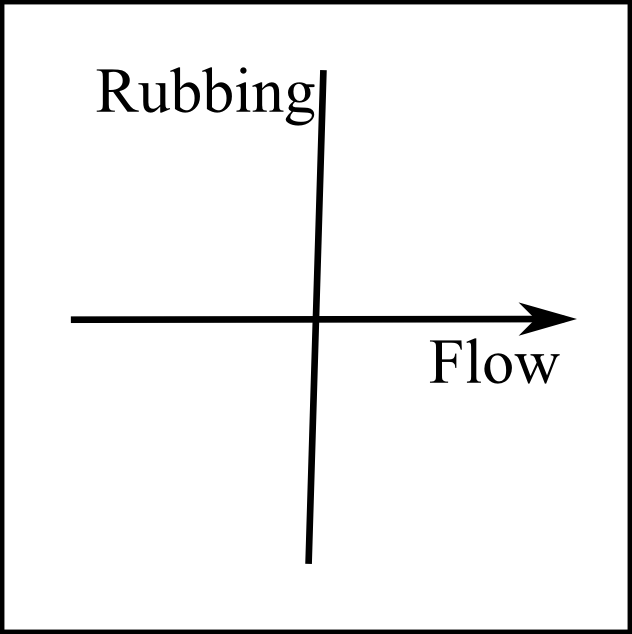
\includegraphics[width=0.3\textwidth]{Figures/Theory/coords}
\end{center}
\caption[Coordinate system]{\label{fig:coords}Coordinate system used throughout this thesis. The tilt angle $\theta$ is defined to be measured from the $z$ axis and the twist angle $\phi$ is defined to be the angle between the projection of $\mathbf{n}$ on to the $x-y$ plane and the $x$ axis}
\end{figure}

In this section, the theory of nematic liquid crystal \textit{flow-alignment} is introduced. That is, the response of the director $\mathbf{n}$ to a velocity gradient. However, to begin with, it is pertinent to pose the question, \textit{``How do we intuitively expect the nematic director to respond to a velocity field?"}

In order to answer this question, a simplified picture of nematic liquid crystal molecules under flow is introduced. This is done by firstly imagining that rather than having molecules flowing in a well defined channel, we replace the channel walls with river banks, and secondly by imagining that rather than having rod-like liquid crystalline molecules, we replace them with wooden logs. If one pictures the flow of a nematic liquid crystal as being directly analogous to the flow of logs in a river (Figure \ref{fig:logging}), a simple, intuitive and useful picture can be formulated in the reader's mind, which will help during later stages in visualising the director's response under complex flow geometries.

\begin{figure}
\begin{center}
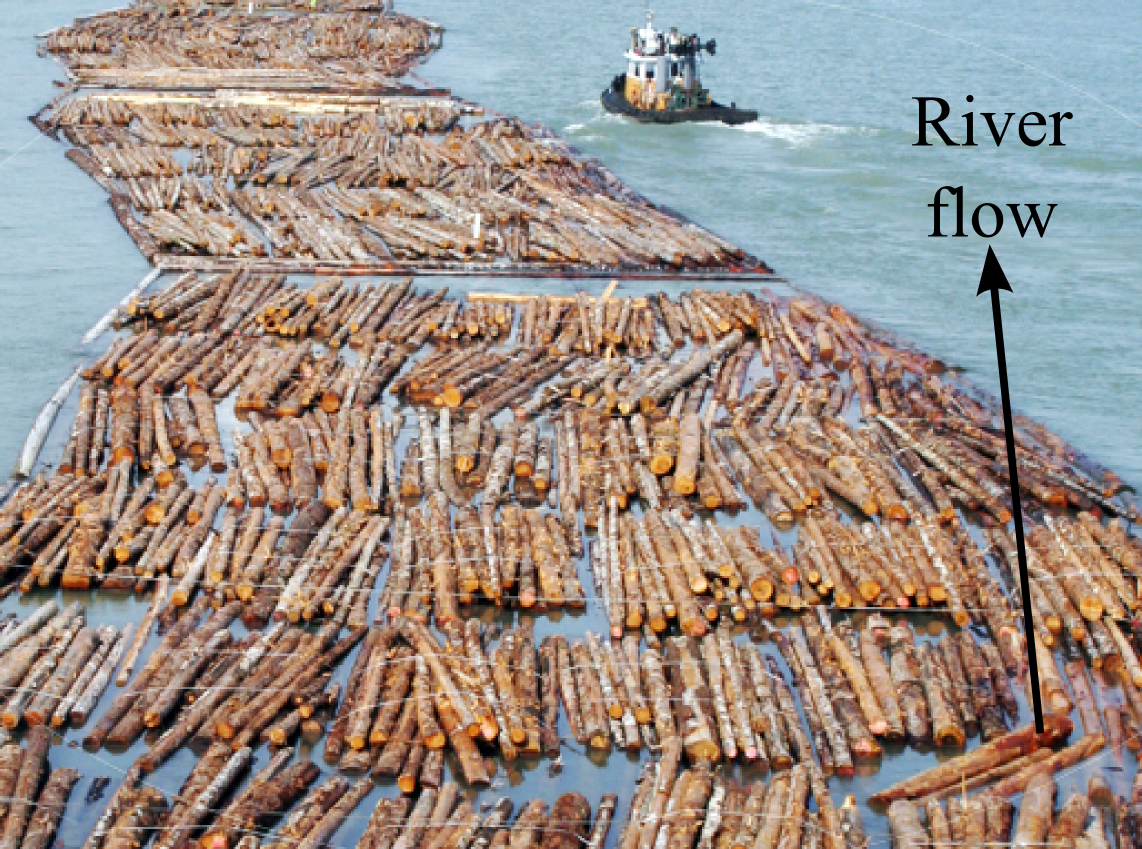
\includegraphics{Figures/Theory/river}
\end{center}
\caption[`Timber being floated to Vancouver, Canada']{\label{fig:logging} `Timber being floated to Vancouver, Canada'. This photograph illustrates how the idea of logs in a river can greatly aid the visualisation of nematic flow-alignment. Here, individual logs are considered the analogue of calamitic liquid crystal molecules, with one long and two short axes. The photograph is licensed under the Creative Commons Attribution 2.0 Generic license and can be found at \href{http://en.wikipedia.org/wiki/File:Log_driving_in_Vancouver.jpg}{http://en.wikipedia.org/wiki/File:Log\_driving\_in\_Vancouver.jpg}}
\end{figure}

It is clear that the three Miesowicz viscosity geometries pictured in Figure \ref{fig:eta} can equally be represented by wooden logs flowing in Figure \ref{fig:logging}. This could be achieved by constraining the logs to have specific orientations with respect to the river velocity and river velocity gradient. Here, the orientation shown in Figure \ref{fig:logging} is equivalent to that of $\eta_1$, where $\mathbf{n}\parallel v$. 

Perhaps intuitively one may expect the director, in response to flow, to azimuthally align itself parallel to the flow direction, as is depicted in Figure \ref{fig:logging}. It seems natural to assume that logs in a river will flow \textit{more easily} in this orientation $\left(\phi=0^{\circ}\right)$. As for the zenithal orientation of the director, again, flow with the logs in planar alignment $\left(\theta=90^{\circ}\right)$ (as in Figure \ref{fig:logging}) naturally feels to be the orientation under which the logs will flow most easily.

As we shall see in the next section, this simplified picture is not entirely incorrect, particularly with respect to the preferred azimuthal orientation of $\phi=0^{\circ}$, providing a very intuitive picture to refer to when analysing more complex flow geometries. Perhaps most interestingly, it will also be shown that for a certain class of liquid crystal, a tilt angle of $\theta=90^{\circ}$ is not the preferred orientation under flow, but that it is rather some small angle away from planar, at which point, the net viscous torque on the nematic molecules goes to zero.

\subsection{Simplified flow-alignment}
In order to gain a basic understanding of the nematic director's response to a flow field, a highly simplified, and in some respects, unrealistic scenario is considered. In this scenario, all effects of boundaries, external fields, director gradients and elastic energies are ignored, leaving only the influence of a linear velocity gradient in $z$ to be considered.

For such a simplified system, the Ericksen-Leslie dynamic equations reduce to two equations, governing the time derivative of $\theta$, $\left(\dot{\theta}=d\theta/dt\right)$ and the time derivative of $\phi$, $\left(\dot{\phi}=d\phi/dt\right)$ \cite{Stewart2004}. These equations describe the orientation of $\mathbf{n}$ for the simplest of shear flow regimes, which apply strictly only under the conditions stated above. These equations are given below (\ref{eq:theta_s} and \ref{eq:phi_s}).

\begin{eqnarray}
\gamma_1\dot{\theta}&=&k\left(\alpha_3\sin^2\theta-\alpha_2\cos^2\theta\right)\cos\phi\label{eq:theta_s}\\
\gamma_1\cos\theta\dot{\phi}&=&k\alpha_3\sin\theta\sin\phi\label{eq:phi_s}
\end{eqnarray}

\noindent As explained by Stewart \cite{Stewart2004}, it is natural to then proceed by seeking steady state solutions to both equations \ref{eq:theta_s} and \ref{eq:phi_s}. That is to ask, \textit{``what values of $\theta$ and $\phi$ are the steady values under shear flow?''} This question is answered by setting $\dot{\theta}=\dot{\phi}=0$, i.e. solving both equations in the condition that the director has stopped rotating, or achieved steady state alignment.

Therefore it is seen that for any values of the viscosities (bearing in mind the equivalence of $\mathbf{n}$ and $-\mathbf{n}$, there is always the steady state alignment provided by

\begin{equation}
\theta=90^{\circ},\hspace{0.5cm}\phi=90^{\circ}
\label{eq:ss_1}
\end{equation}

\noindent These steady state alignment angles correspond to the director being planar $\left(\theta=90^{\circ}\right)$, and lying normal to the flow direction $\left(\phi=90^{\circ}\right)$, as depicted in Figure \ref{fig:ss} (a). Intuitively, this stable alignment condition makes sense. If there is no component of the director in the $z$ direction, then there is no torque acting on the molecules, and therefore there is no torque imbalance, leading to a steady state alignment angle. For a nematic liquid crystal oriented normal to the flow and planar, there is no rotation of the director caused by a shear flow.

However, it can be seen that if the Leslie viscosities $\alpha_2$ and $\alpha_3$ are non-zero and have the same sign, such that $\alpha_2\alpha_3>0$, other possible steady state solutions are provided by

\begin{equation}
\theta=\theta_l,\hspace{0.5cm}\phi=0^{\circ}
\label{eq:ss_2}
\end{equation}

\noindent where the angle $\theta_l$ is referred to as the Leslie angle or \textit{flow alignment angle}, and is calculated from equation \ref{eq:Leslie_angle}, below.

\begin{eqnarray}
\nonumber\alpha_3\sin^2\theta&=&\alpha_2\cos^2\theta\\
\nonumber\tan^2\theta&=&\frac{\alpha_2}{\alpha_3}\\
\theta&=&\tan^{-1}\sqrt{\alpha_2/\alpha_3}\label{eq:Leslie_angle}\\
\theta_l&=&90-\theta\label{eq:conv}
\end{eqnarray}

\noindent Note that the Leslie angle is conventionally defined as a deviation out of the $x-y$ plane, hence the inclusion of equation \ref{eq:conv} to convert our angle into the conventional form. Now it is seen that there is a second set of steady state alignment angles for the director. These constrain the director to be aligned parallel to the direction of flow $\left(\phi=0^{\circ}\right)$, but crucially, not planar aligned $\left(\theta\neq90^{\circ}\right)$, but at some small angle $\left(90-\theta_l\right)$ away from planar, as is demonstrated in Figure \ref{fig:ss} (b).

\begin{figure}
\begin{center}
\subfigure[$\theta=90,\hspace{0.5cm}\phi=90$]{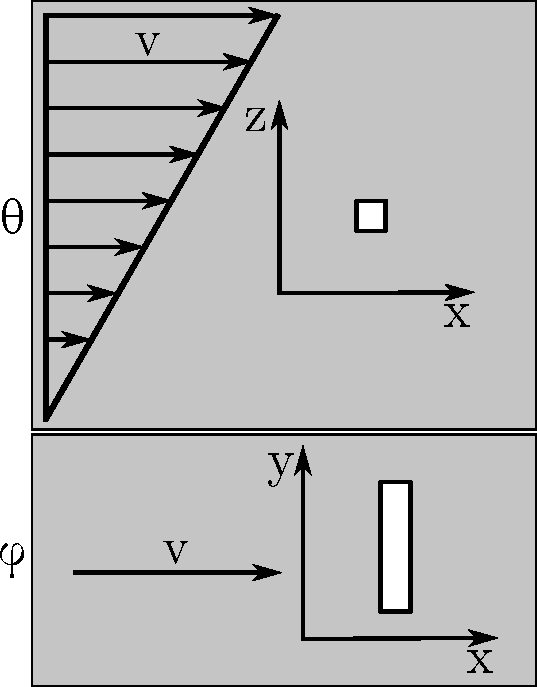
\includegraphics[width=0.2\textwidth]{Figures/Theory/ss_1}}\hspace{0.2in}
\subfigure[$\theta=\theta_l,\hspace{0.5cm}\phi=0$]{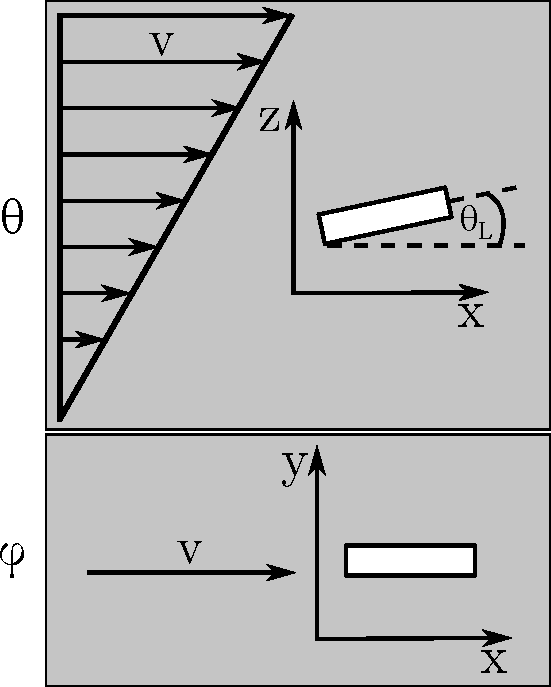
\includegraphics[width=0.2\textwidth]{Figures/Theory/ss_2}}
\end{center}
\caption[Steady state alignment angles of a nematic liquid crystal]{\label{fig:ss} Visual schematic depictions of the steady state alignment angles available to the director under a highly simplified shear flow. (a) shows the alignment angles of $\theta=90^{\circ}$ and $\phi=90^{\circ}$, which are available for any values of the Leslie viscosities. (b) shows the alignment angles of $\theta=\theta_l$ and $\phi=0^{\circ}$, which are only available for \textit{flow-aligning} liquid crystals $\left(\alpha_2\alpha_3>0\right)$.}
\end{figure}

Importantly, if the values of $\alpha_2$ and $\alpha_3$ differ in sign, the only steady state solutions under flow are those given by equation \ref{eq:ss_1}. This follows from equation \ref{eq:Leslie_angle}, where the steady state alignment angle for $\theta$ would involve the square-root of a negative number. Therefore, two classes of liquid crystal can be defined.

\begin{itemize}
\item \textit{Flow-aligning} liquid crystals; where $\alpha_2\alpha_3>0$
\item \textit{Non flow-aligning} liquid crystals; where $\alpha_2\alpha_3<0$
\end{itemize}

\noindent It follows that for flow-aligning liquid crystals, there are two further sub-categories which depend on the relative strengths of $\alpha_2$ and $\alpha_3$, which comes from the thermodynamic constraint that $\gamma_1=\alpha_3-\alpha_ 2>0$, defined by,

%\begin{enumerate}[(I)]
%\item$\alpha_2<\alpha_3<0\hspace{0.5cm}\textrm{where}\hspace{0.5cm}0^{\circ}<\theta_l<45^{\circ},\hspace{0.5cm}\phi=0^{\circ}$
%\item$\alpha_3>\alpha_2>0\hspace{0.5cm}\textrm{where}\hspace{0.5cm}45^{\circ}<\theta_l<90^{\circ},\hspace{0.5cm}\phi=0^{\circ}$
%\end{enumerate}
\begin{equation}
\textrm{Type I}\hspace{0.3cm}\alpha_2<\alpha_3<0\hspace{0.5cm}\textrm{where}\hspace{0.5cm}0^{\circ}<\theta_l<45^{\circ},\hspace{0.5cm}\phi=0^{\circ}
\end{equation}

\begin{equation}
\textrm{Type II}\hspace{0.3cm}\alpha_3>\alpha_2>0\hspace{0.5cm}\textrm{where}\hspace{0.5cm}45^{\circ}<\theta_l<90^{\circ},\hspace{0.4cm}\phi=0^{\circ}
\end{equation}

\noindent Here we see that for $\alpha_2<\alpha_3<0$, the steady state Leslie angle will be valued somewhere between $\theta=90^{\circ}$ and $\theta=45^{\circ}$, which is a relatively small angular deviation away from planar alignment. Conversely, in the case of $\alpha_3<\alpha_2>0$, the Leslie angle will be valued between $\theta=45^{\circ}$ and $\theta=0^{\circ}$, which is a relatively large distortion away from planar alignment. It is purely this torque balance, created by the differing relative strengths of $\alpha_2$ and $\alpha_3$ which create the steady state Leslie angle.

The values of the Leslie viscosity coefficients for three common nematic liquid crystals are given in Table \ref{tab:visc}. It can be seen for the experimental viscosities given in Table \ref{tab:visc}, that 5CB, MBBA and PAA are all Type I \textit{flow-aligning}.

\begin{table}[ht]
\centering  % used for centering table
\begin{tabular}{l|c|cccccc} 
\hline\hline                       
&&\multicolumn{6}{c}{\textbf{Leslie Viscosity (Pa.s)}}\\
Liquid Crystal&T $^{\circ}$C&$\alpha_1$&$\alpha_2$&$\alpha_3$&$\alpha_4$&$\alpha_5$&$\alpha_6$\\
\hline                  
5CB &$25^{\circ}$& -0.0060& -0.0812&-0.0036&0.0652&0.0640&-0.0208\\
MBBA& $25^{\circ}$&-0.0181&-0.1104&-0.0011&0.0826&0.0779&-0.0336\\
PAA& $122^{\circ}$&0.0043&-0.0069&-0.0002&0.0068&0.0047&-0.0023\\
\hline
\end{tabular}
\caption[Values of the Leslie viscosities for the nematic phases of 5CB, MBBA and PAA]{Values of the Leslie viscosities for the nematic phases of 5CB, MBBA and PAA (taken from reference \cite{Stewart2004}). Note that all three nematic phases are flow-aligning.} 
\label{tab:visc}
\end{table}

After this introduction to the theoretical background of nematic liquid crystal dynamics, this chapter will now go on to introduce and examine the workings of the one dimensional model that is used to simulate director dynamics in liquid crystal cells undergoing pressure driven flow in well defined flow channels.

\newpage

\subsection{A 1-D numerical model of liquid crystal dynamics}
This section introduces the one dimensional model of liquid crystal dynamics that is used extensively in later chapters of this thesis. The rigorous and full details of the model's design and operation are provided by its creator, Stephen Cornford, in his thesis ``Recovery and analysis of director profiles in liquid crystal cells'' \cite{Cornford2008} where a substantial amount of effort has gone into creating the model and comparing its output to other simulation packages available (such as DIMOS). As is described in reference \cite{Cornford2008}, although other computer programs that can model simple liquid crystal cells have been used before in the Exeter group \cite{Birkett2008,Jewell2002}, this model was created in order to compute the dynamics of rather more complex situations including simulation of the flexo-electric effect, ion motion in cells, use in optimisation problems and, most importantly in the context of this thesis, the effects of pressure-driven flow upon director distortion.

This section aims to provide a brief introduction to the key equations of the model which govern the dynamic behaviour that will be seen in later experimental chapters of this thesis. In addition to that, this section also intends to give a brief introduction to how the model is used in this thesis, including what difficulties have been overcome in order for it to operate.
 
\subsubsection{Assumptions}
The dynamical behaviour of the liquid crystal described by this one dimensional model is governed by the Leslie-Ericksen equations (as introduced earlier in this chapter). That is to say, the model is derived from the continuum theory of nematic liquid crystals, where the liquid crystal is described by a director field \cite{Cornford2008}.

For a simple cell, the liquid crystal can be described by this director field $\mathbf{n}\left(z,t\right)$, and a flow field $\mathbf{u}\left(z,t\right)$. Given this assumption, the model is based upon a Cartesian co-ordinate system that has been chosen so the cell walls (upper and lower) lie parallel to the $xy$ plane at $z=0$ and $z=d$. As this is only a one dimensional simulation, the cell is also assumed to be infinitely large in both the $x$ and $y$ directions so that only variations in the director parallel to the $z$ axis need to be considered \cite{Cornford2008}. As was described at the start of Section \ref{sec:logs} (Figure \ref{fig:coords}), the Euler angles $\theta\left(z,t\right)$ and $\phi\left(z,t\right)$ are used to specify the director $\mathbf{n}$. As is traditional in the Exeter group, the tilt angle $\theta$ is defined to be measured from the $z$ axis and the twist angle $\phi$ is defined to be the angle between the projection of $\mathbf{n}$ on to the $x-y$ plane and the $x$ axis, expressed as

\begin{equation}
\mathbf{n}=\left(\sin\theta\cos\phi,\sin\theta\sin\phi,\cos\theta\right)
\end{equation}

Another result of the one dimensional assumption is that only two variables $u_x$ and $u_y$ are needed to fully describe the nature of $\mathbf{u}$. As is detailed in \cite{Cornford2008} the basis for this assumption is made clear when $\mathbf{u}$ is taken to be defined by

\begin{equation}
\mathbf{u}=\left(u_x,u_y,u_z\right)
\end{equation}

\noindent As the flow is assumed to be incompressible, $\nabla\cdot\mathbf{u}=0$. If the flow field \textit{varies} only in $z$, this divergence equality reduces to 

\begin{equation}
\frac{\partial u_z}{\partial z}=0
\end{equation}

\noindent Since there is no flow through the top and bottom walls of the cell, $u_z\left(0\right)=u_z\left(d\right)=0$, and therefore $u_z$ must equal zero, and hence there is only the requirement for two variables $u_x$ and $u_y$ to fully describe $\mathbf{u}$.

It is worth noting that as well as the director and flow fields described above, the electric field $\mathbf{E}$ within the cell must be taken into account if simulations involving the effects of an applied electric potential are also to be considered\footnote{The model described here takes into account the possibility of an applied electric field through ITO coated substrates, the flexoelectric effect or space charges.}. In such a case, the electric displacement vector $\mathbf{D}$, must be constant in a one dimensional system \cite{Cornford2008}. As $\mathbf{D}$ is confined to be parallel to the $z$ axis at the cell boundaries, it must therefore be parallel to $z$ at all points in the cell and hence only components of $\mathbf{E}$ parallel to the $z$ axis are considered in the simulation equations.

\subsection{The Leslie-Ericksen equations}
The time and space dependent behaviour of $\mathbf{n}$ and $\mathbf{u}$ can be found by solving the Leslie-Ericksen equations. These equations boil down to four partial differential equations in the variables $\theta,\space\phi,\space u_x$ and $u_y$. Prior to examining these equations, some auxiliary functions of $\theta$ are defined for convenience \cite{Cornford2008}

\begin{eqnarray}
a\left(\theta\right)&=&\left(\alpha_6+\alpha_3+2\alpha_1\cos^2\theta\right)\sin^2\theta\\
b\left(\theta\right)&=&\left(\alpha_5-\alpha_2\right)\cos^2\theta+\alpha_4\\
c\left(\theta\right)&=&\alpha_3\sin^2\theta-\alpha_2\cos^2\theta\\
\label{eq:c}
g\left(\theta\right)&=&\sin^2\theta\left(\left(k_{22}-k_{33}\right)\sin^2\theta+k_{33}\right)\\
g^\prime\left(\theta\right)&=&\frac{dg}{d\theta}
\end{eqnarray}

\subsubsection{Twist}
\label{sec:phi}

The governing equation for the azimuthal angle $\phi$ is derived from \cite{Cornford2008} and \cite{Stewart2004},

\begin{widetext}
\begin{equation}
\gamma_1 \sin^2\theta\frac{d\phi}{dt}=g\left(\theta\right)\frac{\partial^2\phi}{\partial z^2} + 
g'\left(\theta\right)\frac{\partial\theta}{\partial z}\frac{\partial\phi}{\partial z}- \\
\frac{1}{2}\alpha_2\sin2\theta\left(\cos\phi\frac{\partial u_y}{\partial z}-\sin\phi\frac{\partial u_x}{\partial z}\right)
\label{eq:phi}
\end{equation}
\end{widetext}

\noindent Boundary conditions and initial conditions for equation \ref{eq:phi} must be provided, giving $\phi\left(z=0,t=0\right)$, $\phi\left(z=d,t=0\right)$ and $\phi\left(z,t=0\right)$. That is, the initial azimuthal director alignment has to be provided. Generally, when simulating the response of a cell, the angles in the simulation will be those of the rubbing direction on the actual cell.

If a uniform $\left(d\phi/dz=0\right)$, planar aligned $\left(\theta=90^{\circ}\right)$ sample were to be considered, it is seen that all terms in equation \ref{eq:phi} equal zero. That is to say, if a liquid crystal sample were to be held planar, there would be no azimuthal distortion of the director under flow (the same is also true for $\theta=0^{\circ}$). However, if there were to be a small amount of tilt of the director introduced to the cell $\left(\theta\neq90\right)$, the third term in equation \ref{eq:phi},

\begin{equation}
\frac{1}{2}\alpha_2\sin2\theta\left(\cos\phi\frac{\partial u_y}{\partial z}-\sin\phi\frac{\partial u_x}{\partial z}\right)
\end{equation}

\noindent will no longer equal zero, and azimuthal rotation of the director will be simulated with the onset of flow. This result is important, and ties in with the more qualitative explanation of azimuthal rotation which is described later in Chapter \ref{cha:45}.

Another important point to note about equation \ref{eq:phi} is that in steady state, where $d\phi/dt=0$, (ignoring the contribution from $u_y$) $\sin\phi\left(\partial u_x/\partial z\right)$ in the final term must also equal zero. Given that under flow $\partial u_x/\partial z$ will not equal zero, then the value of $\sin\phi$ must equal zero, yielding steady state values of $\phi=0^{\circ},180^{\circ}$, or the director lying parallel to the $x$ axis (flow direction). Therefore, considering the more involved equations describing the dynamic behaviour of a nematic liquid crystal under pressure driven flow between two parallel plates, the same steady state azimuthal alignment angles of the director are recovered, as were seen earlier for the highly simplified case in the azimuthal component of equation \ref{eq:ss_2}.

\subsection{Tilt}
A similar governing equation for the zenithal (tilt) angle $\theta$ is derived from \cite{Cornford2008} and \cite{Stewart2004},

\begin{eqnarray}
\nonumber \gamma_1\frac{\partial\theta}{\partial t} & = & \left(k_{11}+\left(k_{33}-k_{11}\right)\cos^2\theta\right)\frac{\partial^2\theta}{\partial z^2}\\
\nonumber	& & {} + \frac{1}{2}\left(k_{11}-k_{33}\right)\sin2\theta\left(\frac{\partial\theta}{\partial z}\right)^2\\
\nonumber	& & {} + \frac{1}{2}g'\left(\theta\right)\left(\frac{\partial\phi}{\partial z}\right)^2+c\left(\theta\right)\left(\cos\phi\frac{\partial 							u_x}{\partial z}+\sin\phi\frac{\partial u_y}{\partial z}\right)\\
	& & {} + \frac{1}{2}\sin2\theta\left(\left(e_s-e_b\right)\frac{\partial E}{\partial z}-\epsilon_0\epsilon_aE^2\right)
	\label{eq:theta}
\end{eqnarray}

Again, boundary conditions for equation \ref{eq:theta} must be provided, giving $\theta\left(z=0,t=0\right)$, $\theta\left(z=d,t=0\right)$ and $\theta\left(z,t=0\right)$. That is, the initial tilt director alignment has to be provided, again, this is provided physically by the type of surface alignment layer that is deposited on cell walls.

Here, in steady state and assuming a uniform alignment $\left(\partial\theta / \partial t=0\right)$, $c\left(\theta\right)$ must equal zero, which from equation \ref{eq:Leslie_angle} is shown to occur at the Leslie angle.

\subsection{Flow field}
The last two governing equations are those for the simulated flow field and are derived from the linear momentum balance equations \cite{Cornford2008} where the pressure gradients $G_x$ and $G_y$ are defined along the $x$ and $y$ axes respectively. These are given in \ref{eq:Gx} and \ref{eq:Gy} below.

It is worth noting that the only time derivatives contained in equations \ref{eq:Gx} and \ref{eq:Gy} are those of $\theta$ and $\phi$. This dictates that if the director is not changing in time, the flow fields are also time independent. 
Consequently, only boundary conditions for $u_x$ and $u_y$ must be prescribed. As will also be discussed later, the classical non-slip boundary condition stating that the fluid velocity at the cell walls is assumed to be zero is appropriate \cite{Cornford2008,Feynmann1964}.

\begin{align}
G_x &= \frac{\partial}{\partial z}\left(\left[\frac{1}{2}a\left(\theta\right)\cos^2\phi+b\left(\theta\right)\right]\frac{\partial u_x}{\partial z} \right. \nonumber \\
&+\frac{1}{4}a\left(\theta\right)\sin2\phi\frac{\partial u_y}{\partial z} \nonumber \\
&-c\left(\theta\right)\cos\phi\frac{\partial \theta}{\partial t} \nonumber \\
&\left.-\frac{1}{2}\alpha_2\sin\phi\sin2\theta\frac{\partial \phi}{\partial t}\right)
\label{eq:Gx}
\end{align}

\begin{align}
G_y &= \frac{\partial}{\partial z}\left(\left[\frac{1}{2}a\left(\theta\right)\sin^2\phi+b\left(\theta\right)\right]\frac{\partial u_y}{\partial z} \right. \nonumber \\
&+\frac{1}{4}a\left(\theta\right)\sin2\phi\frac{\partial u_x}{\partial z} \nonumber \\
&-c\left(\theta\right)\sin\phi\frac{\partial \theta}{\partial t} \nonumber \\
&\left.-\frac{1}{2}\alpha_2\cos\phi\sin2\theta\frac{\partial \phi}{\partial t}\right)
\label{eq:Gy}
\end{align}

% 
% \begin{equation}
% G_x = \frac{\partial}{\partial z}\left(\left[\frac{1}{2}a\left(\theta\right)\cos^2\phi+b\left(\theta\right)\right]\frac{\partial u_x}{\partial z}
% +\frac{1}{4}a\left(\theta\right)\sin2\phi\frac{\partial u_y}{\partial z}-c\left(\theta\right)\cos\phi\frac{\partial \theta}{\partial t}-\frac{1}{2}\alpha_2\sin\phi\sin2\theta\frac{\partial \phi}{\partial t}\right)
% \label{eq:Gx}
% \end{equation}
% 
% 
% \begin{equation}
% G_y = \frac{\partial}{\partial z}\left(\left[\frac{1}{2}a\left(\theta\right)\sin^2\phi+b\left(\theta\right)\right]\frac{\partial u_y}{\partial z}
% +\frac{1}{4}a\left(\theta\right)\sin2\phi\frac{\partial u_x}{\partial z}-c\left(\theta\right)\sin\phi\frac{\partial \theta}{\partial t}-\frac{1}{2}\alpha_2\cos\phi\sin2\theta\frac{\partial \phi}{\partial t}\right)
% \label{eq:Gy}
% \end{equation}

\noindent As a final note, as discussed earlier and shown in equations \ref{eq:phi} and \ref{eq:theta}, the boundary conditions for $\theta$ and $\phi$ are known (from experiment) and are input into the one dimensional model used here. As is explained in \cite{Cornford2008}, it is also reasonable to assume that the director is fixed at the cell surfaces, in a regime known as \textit{strong anchoring}. An alternative regime could also be considered, \textit{weak anchoring} (not used in this simulation) whereby information regarding $\theta$ and its derivative in $z$ and $\phi$ and its derivative in $z$ would be required\footnote{Some relevant material is included in references \cite{Cui2006} and \cite{Choate2008}.}.

Finally, this chapter will go on to introduce the experimental technique of conoscopy as a means of extracting information about nematic liquid crystal alignment. Conoscopy is used widely in later experimental chapters of this thesis and here, a computational method of simulating conoscopic figures is introduced along with some characteristic figures recorded in the experiments.

\newpage
\subsection{Conoscopy}
Conoscopy, from the greek \textit{konos} meaning cone, and \textit{skopeo} meaning examine \cite{wikipedia}, has long been used as a tool for studying the physical nature and alignment of geological crystals and their birefringence. More recently, it has been used to explore liquid crystal mono-domain alignment \cite{Horn2001}. As will be seen later in the experimental chapters of this thesis, conoscopy is also a relatively simple and powerful tool for gaining a large amount of information about a liquid crystal director profile in a relatively quick manner. Not withstanding it's relative speed-of-use and ease of implementation, it does have certain shortcomings when directly compared to more detailed and rigorous analysis methods such as the Fully Leaky Guided Mode (FLGM) technique \cite{Cornford2009,Yang2007,Jewell2005a,Jewell2006,Jewell2007}.

Optical conoscopy, as used in this work, gives a broad (lacking in fine detail) picture of how the director behaves or reacts to an external perturbation such as an applied pressure gradient inducing flow. As such, the aim of conoscopy is not to accurately determine the director profile at a high spatial resolution, but rather to give a broad overview of the alignment present within the cell.

\subsection{Simulation}
Conoscopic `interference' figures are generated when birefringent crystal samples are viewed between crossed polarisers with highly convergent monochromatic light\footnote{White light can also be used}. Essentially, as is well explained by Van Horn and Henning-Winter \cite{Horn2001}, when light rays pass through the crystal, they are split into ordinary and extraordinary components which experience different refractive indices and hence travel along different paths. For liquid crystal mono-domains, these different paths are highly dependent on the degree of order exhibited within the liquid crystal mono-domain. Depending on the phase difference between these rays, light exiting the crystal may have undergone polarisation conversion, resulting in some light in specific directions passing the second, crossed, polariser. For light rays over a cone of angles, characteristic figures are observed, depending on the alignment of the mono-domain that has been traversed.

Figure \ref{fig:con_samples} shows a schematic representation of the common conoscopic figures that are observed for the primary alignment states of the director. For reference, conoscopic figures are said to consist of dark isochromatic fringes, and extinction brushes or \textit{isogyres}. When the director is aligned parallel to the surface (planar, Figure \ref{fig:con_samples} (a)) the conoscopic figure observed is a set of conjugate hyperbolae, centred on a common locus \cite{Horn2001}. Light that has travelled to the centre of the locus (if it is bright) will have passed along a path where the relative phase difference between the ordinary and extraordinary light is a maximum. For vertical director alignment (Figure \ref{fig:con_samples} (b)), the conoscopic figure consists of concentric circular fringes and a central extinction cross. Here, the centre of the cross corresponds to minimum relative phase difference \cite{Horn2001}. For a director profile that is uniformly tilted (Figure \ref{fig:con_samples} (c)), the conoscopic figure consists of a series of dark fringes resulting from the birefringence encountered by light passing through the cell\footnote{The conoscopic images shown in Figure \ref{fig:con_samples} are calculated from the uniaxial modelling script described later}. This conoscopic figure is simulated for a large $\left(\approx45^{\circ}\right)$ uniform tilt angle. For smaller tilt angles, a displacement of the locus from the centre of the field of view is observed, which, as will be seen later, can be used to estimate the tilt angle within the sample.

\begin{figure}
\begin{center}
\subfigure[Planar]{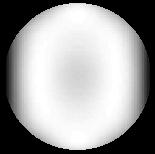
\includegraphics[width=0.3\textwidth]{Figures/conoscopy/1}}
\subfigure[Vertical]{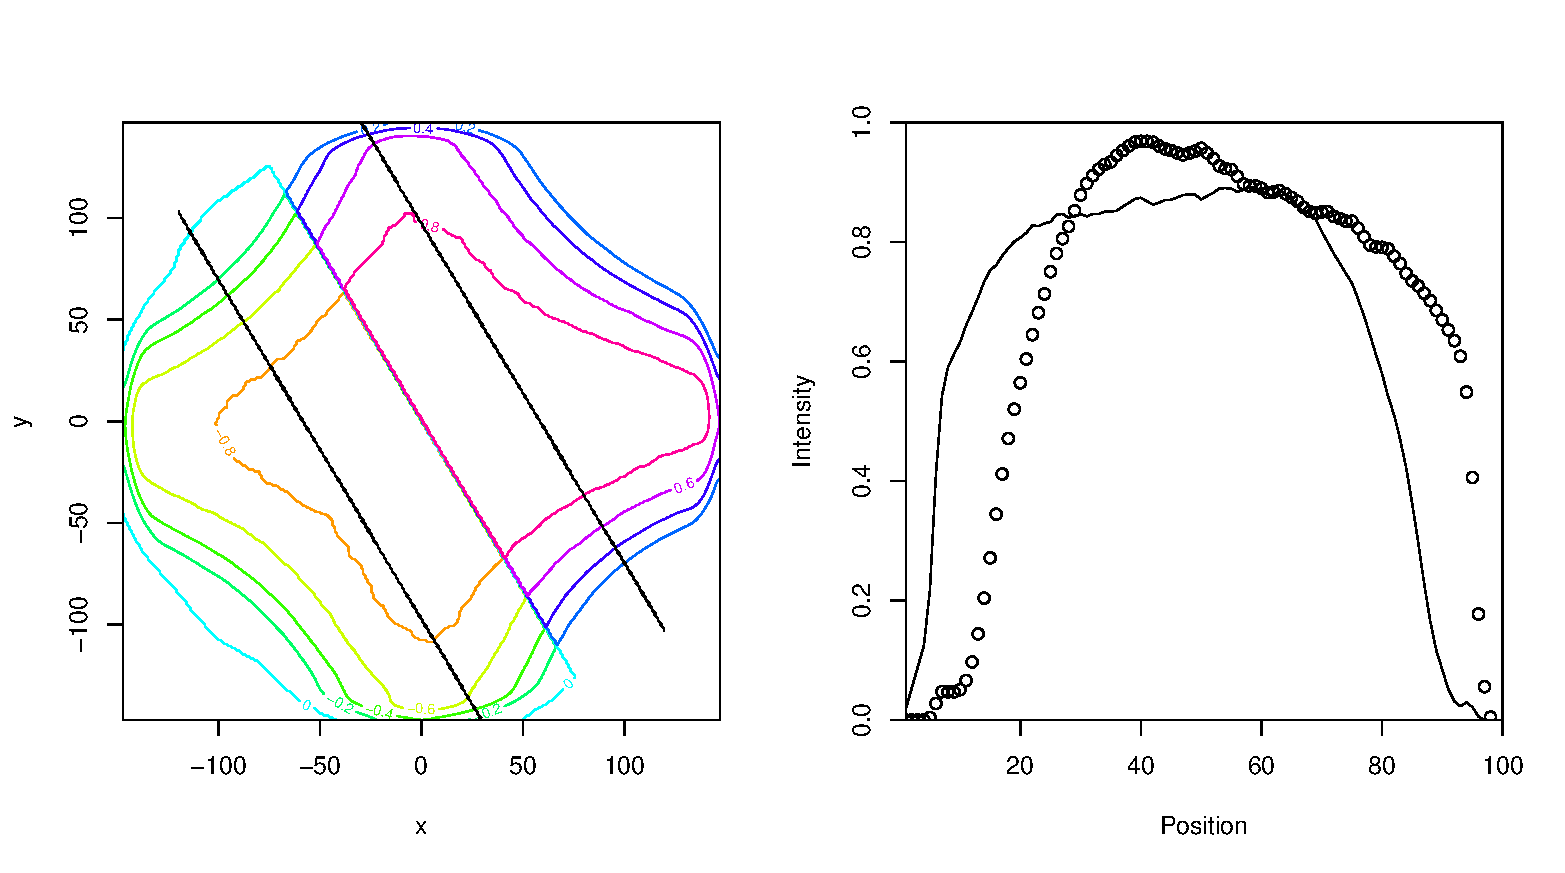
\includegraphics[width=0.3\textwidth]{Figures/conoscopy/2}}
\subfigure[Tilted]{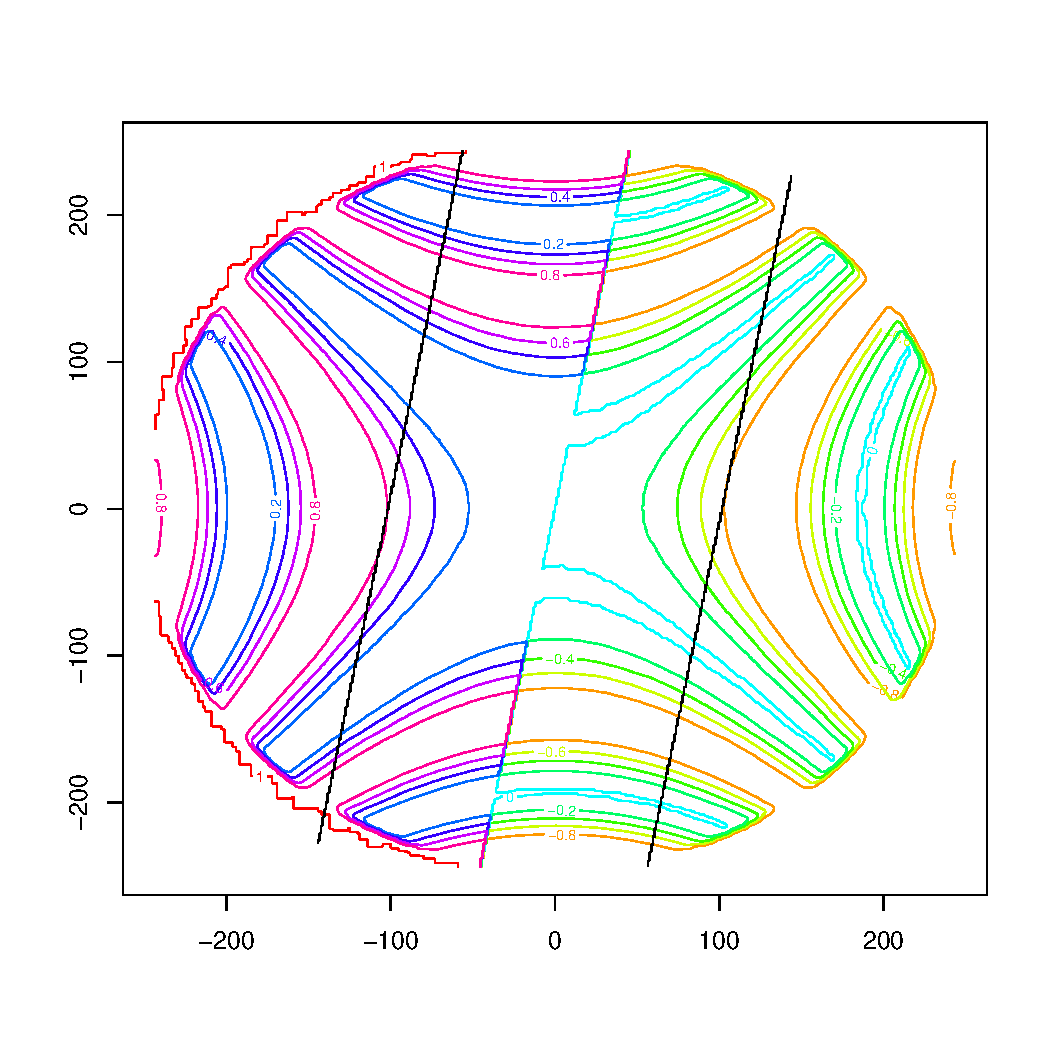
\includegraphics[width=0.3\textwidth]{Figures/conoscopy/3}}
\end{center}
\caption[Simulated conoscopic images for planar, vertical and tilted alignment]{\label{fig:con_samples}Simulated conoscopic figures for the director profiles shown schematically on the left. (a) the double set of hyperbolae signalling planar alignment. (b) The maltese cross from vertical alignment of the director. (c) A series of dark fringes from a uniformly tilted sample.}
\end{figure}

A modelling script was also developed by Stephen Cornford \cite{Cornford2008} in order to simulate the conoscopic figures observed for birefringent media. As used widely in his thesis, the Berreman \cite{Berreman1972} (or Jones) matrix methods were adapted to compute the conoscopic figures, as has been reported previously in the literature \cite{Ogasawara2001,Parry-Jones2002}.

Briefly, a cartesian coordinate system is defined for the computation of the conoscopic figure. Each point within that coordinate system $\left(x,y\right)$ can be defined by a pair of angles $\alpha$ and $\psi$ such that \cite{Cornford2008},

\begin{eqnarray}
\tan\psi=y/x\\
\sin\alpha=\left(x^2+y^2\right)^{\frac{1}{2}}
\end{eqnarray}

A ray of light that passes through the focus of the cone of light at an angle of incidence $\alpha$, strikes the cartesian coordinate system plane with a plane of incidence at angle $\psi$ to the figure's $x$ axis and at an angle $\psi^{\prime}$ to the transmission angle of the polariser. 

For each ray in the cone of incident light, the coefficients $E_{ss},E_{sp},E_{ps},E_{pp}$ are calculated, where $E_{sp}$ is the complex, $s$-polarised component of the electric field transmitted through the sample if the incoming ray were wholly $p$-polarised. From these, the intensity at any point on the cartesian coordinate system can be obtained \cite{Cornford2008} from,

\begin{widetext}
\begin{equation}
I\left(\alpha,\psi\right)=\left|\left(E_{pp}-E_{ps}\right)\sin\left(\psi^{\prime}\right)\cos\left(\psi^{\prime}\right)-E_{ps}\cos^2\psi^{\prime}+E_{sp}\sin^2\psi^{\prime}\right|^2
\end{equation}
\end{widetext}

In order to compute the interference figure, a set of points in the cartesian coordinate plain $\left(x,y\right)$ needs to be selected such that $\sin\alpha\leq\sin\text{NA}$, where NA is the numerical aperture of the cone of light \cite{Cornford2008}.

Figure \ref{fig:figures} shows a table of simulated conoscopic figures from the computational method described above. These figures are simulated for a typical nematic liquid crystal with refractive indices of $n_e=1.7$ and $n_o=1.5$ in  a cell approximately 100 $\mu m$ thick. The sequence of figures correspond to the liquid crystal uniform tilt angle $\theta$ varying along a row, whilst the azimuthal angle $\phi$ varies along a column.

\begin{center}
\begin{table}[ht]
\newcolumntype{C}{>{\centering\arraybackslash} m{1cm}}
\begin{tabular}{ccCCCCC}
&&&&$\theta$&&\\
&&90$^{\circ}$&85$^{\circ}$&45$^{\circ}$&5$^{\circ}$&0$^{\circ}$\\
&\centering{90}$^{\circ}$&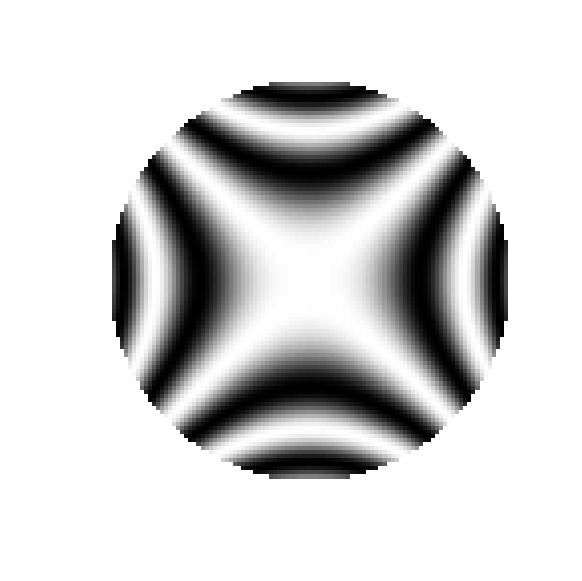
\includegraphics[width=0.06\textwidth]{Figures/conoscopy/table/90_90}&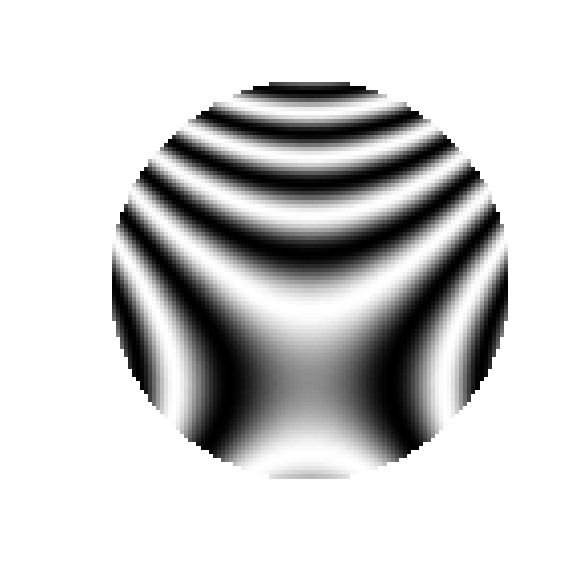
\includegraphics[width=0.06\textwidth]{Figures/conoscopy/table/90_85}&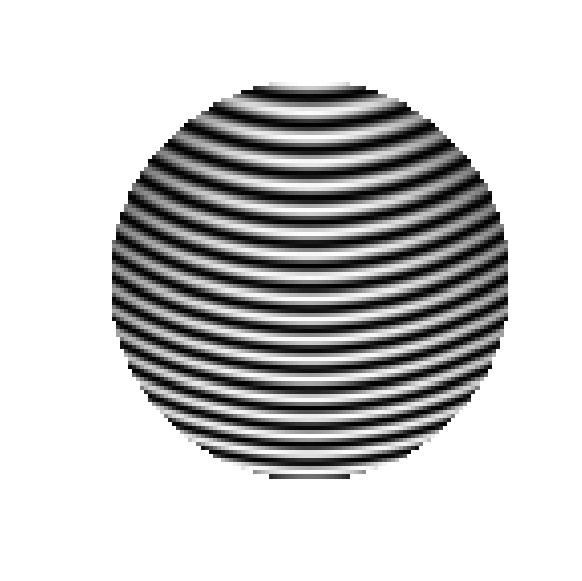
\includegraphics[width=0.06\textwidth]{Figures/conoscopy/table/90_45}&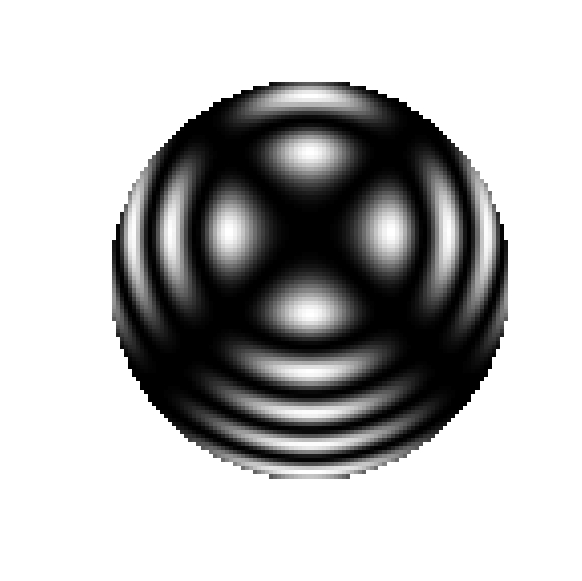
\includegraphics[width=0.06\textwidth]{Figures/conoscopy/table/90_05}&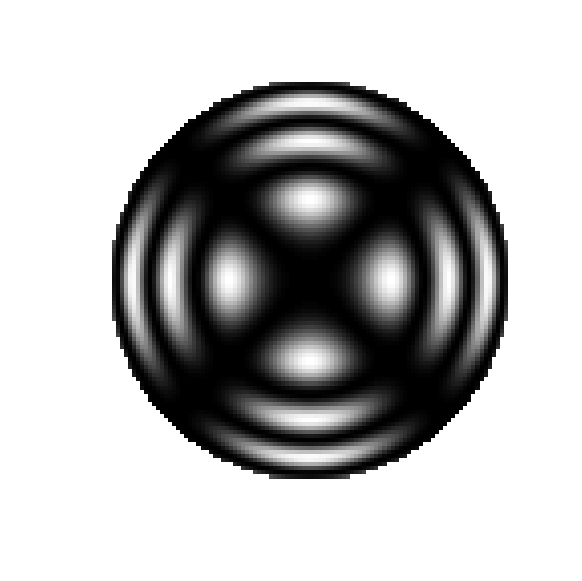
\includegraphics[width=0.06\textwidth]{Figures/conoscopy/table/90_00}\\

&60$^{\circ}$&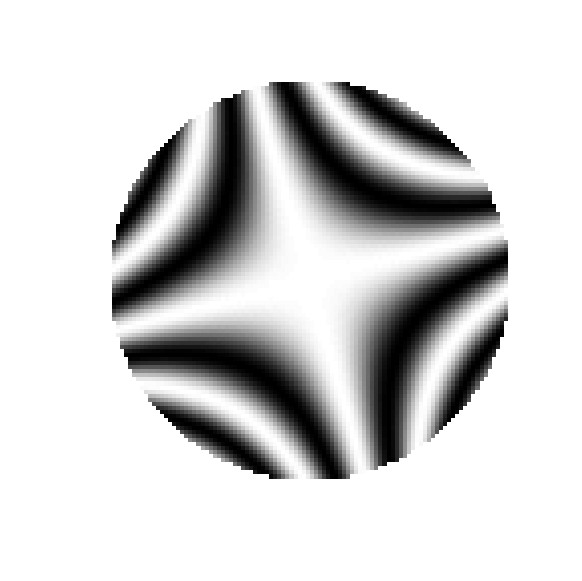
\includegraphics[width=0.06\textwidth]{Figures/conoscopy/table/60_90}&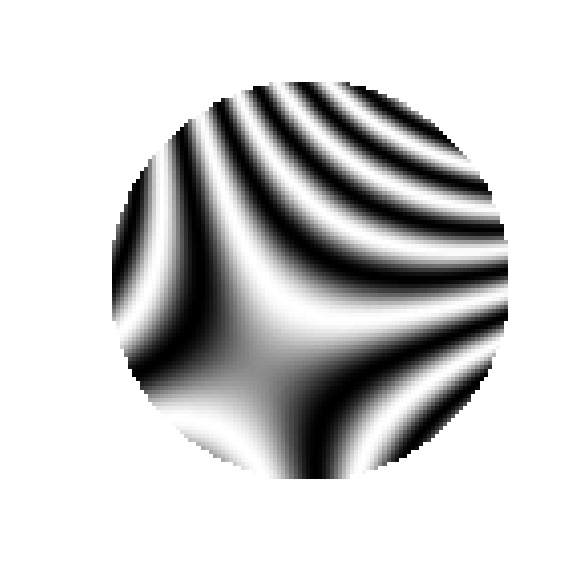
\includegraphics[width=0.06\textwidth]{Figures/conoscopy/table/60_85}&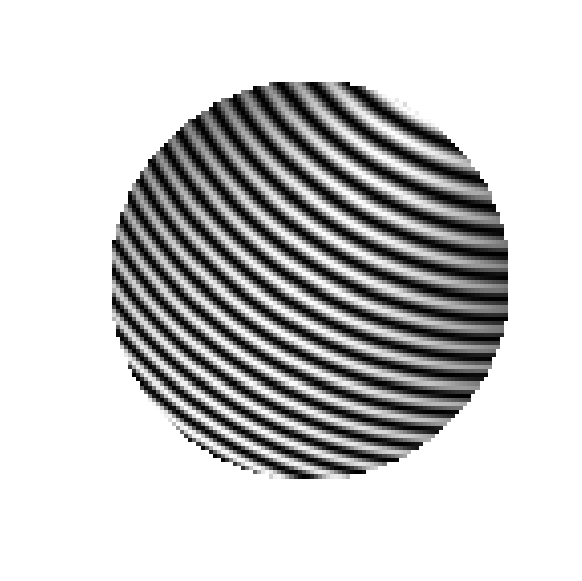
\includegraphics[width=0.06\textwidth]{Figures/conoscopy/table/60_45}&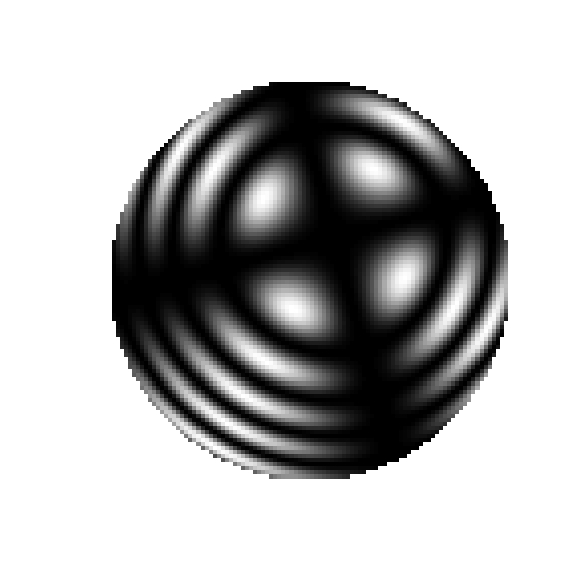
\includegraphics[width=0.06\textwidth]{Figures/conoscopy/table/60_05}&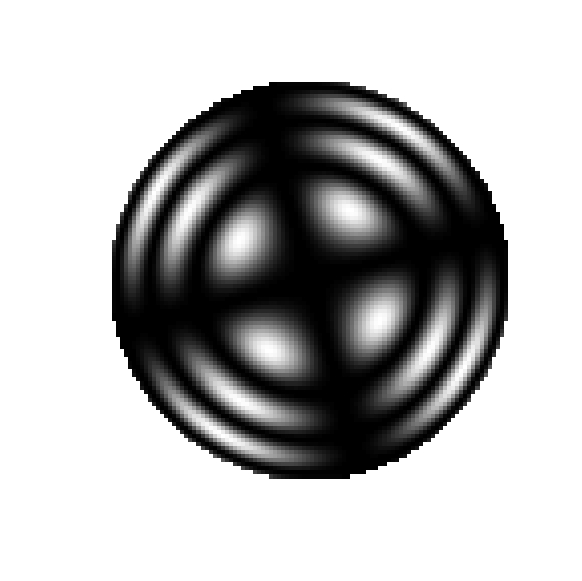
\includegraphics[width=0.06\textwidth]{Figures/conoscopy/table/60_00}\\

$\phi$&45$^{\circ}$&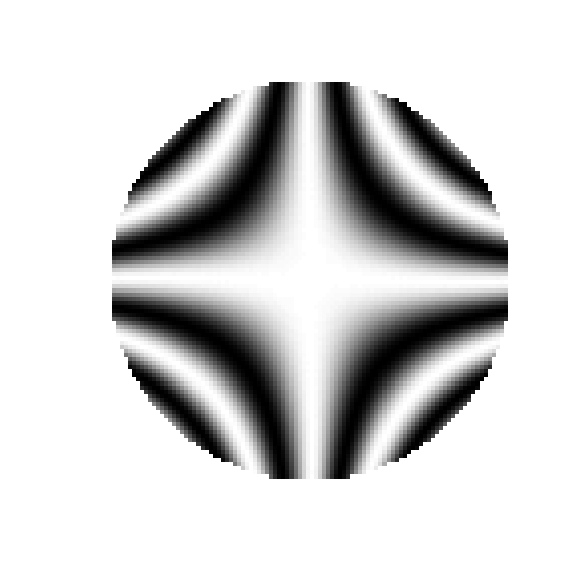
\includegraphics[width=0.06\textwidth]{Figures/conoscopy/table/45_90}&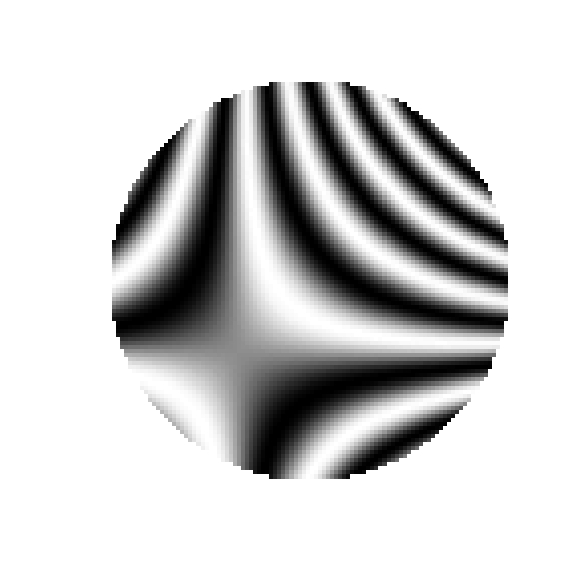
\includegraphics[width=0.06\textwidth]{Figures/conoscopy/table/45_85}&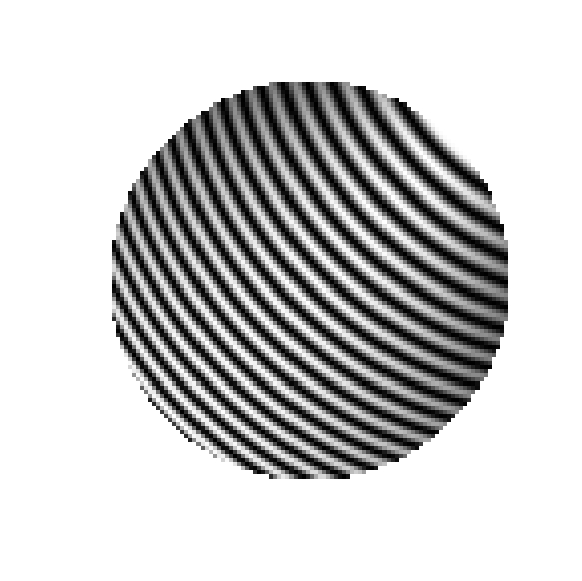
\includegraphics[width=0.06\textwidth]{Figures/conoscopy/table/45_45}&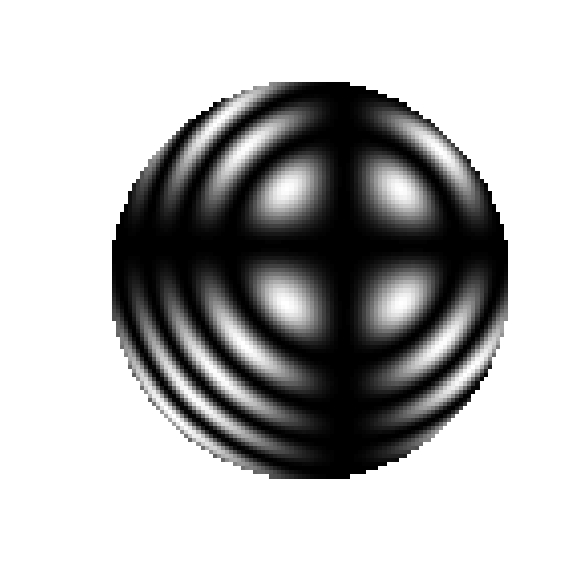
\includegraphics[width=0.06\textwidth]{Figures/conoscopy/table/45_05}&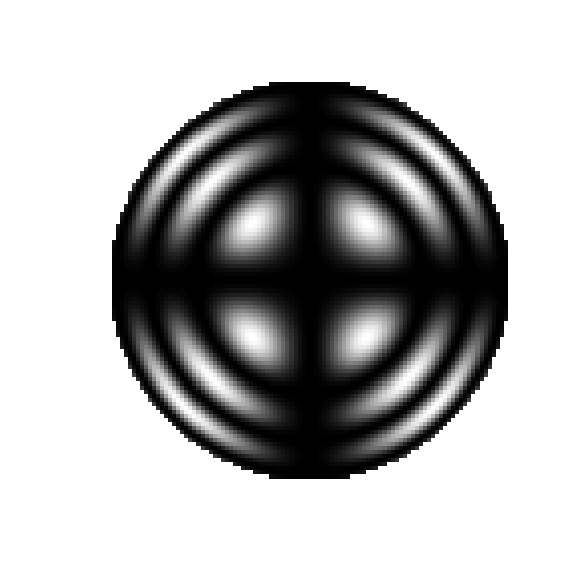
\includegraphics[width=0.06\textwidth]{Figures/conoscopy/table/45_00}\\

&30$^{\circ}$&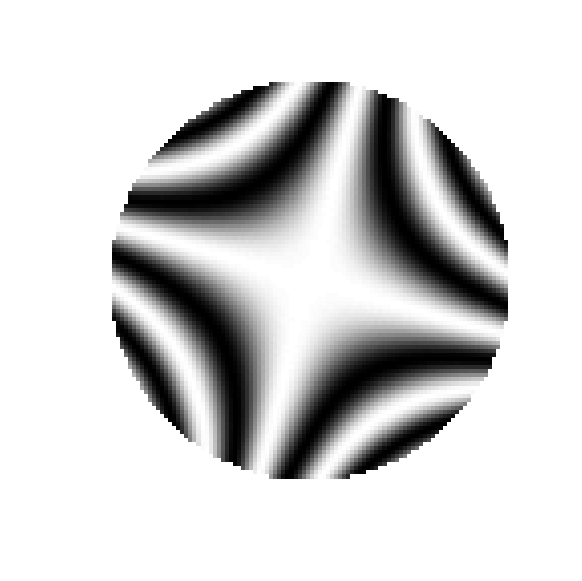
\includegraphics[width=0.06\textwidth]{Figures/conoscopy/table/30_90}&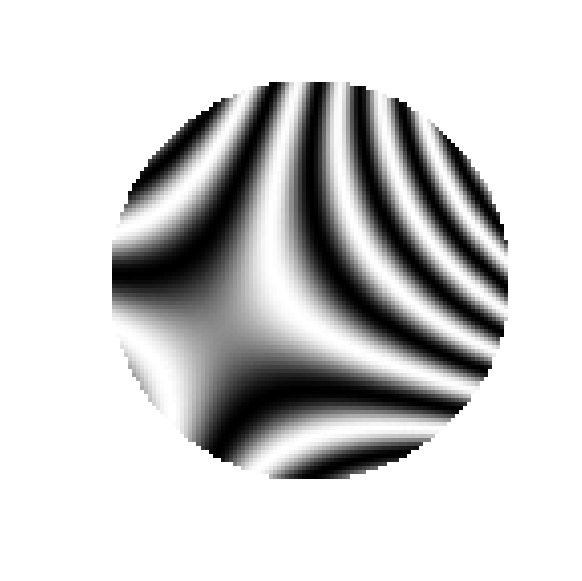
\includegraphics[width=0.06\textwidth]{Figures/conoscopy/table/30_85}&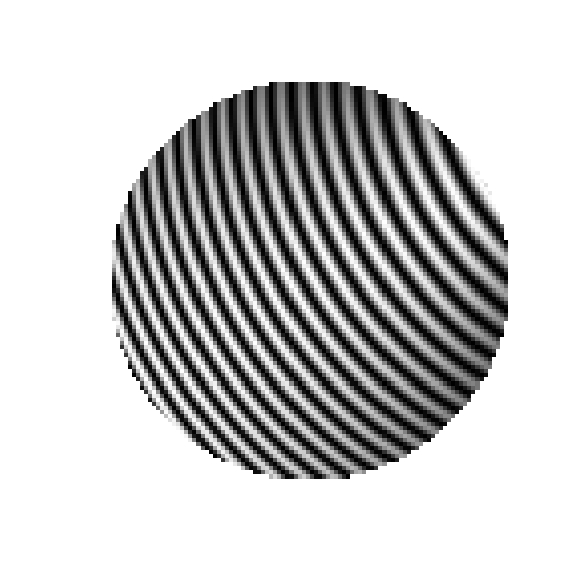
\includegraphics[width=0.06\textwidth]{Figures/conoscopy/table/30_45}&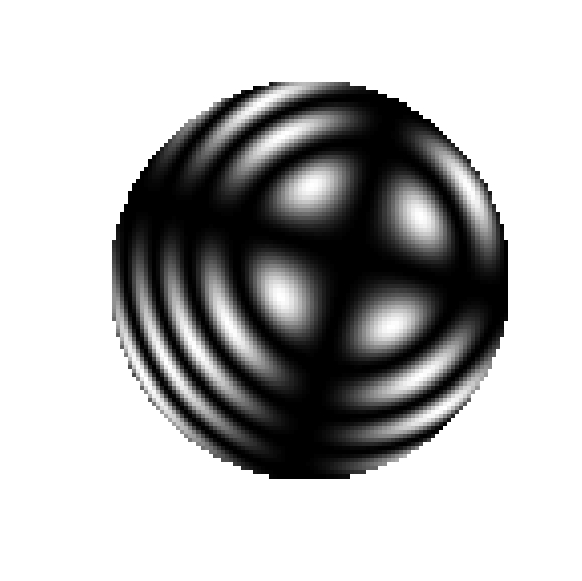
\includegraphics[width=0.06\textwidth]{Figures/conoscopy/table/30_05}&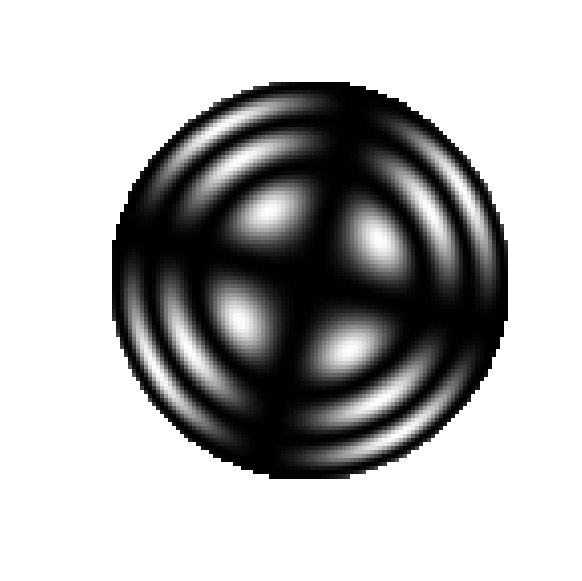
\includegraphics[width=0.06\textwidth]{Figures/conoscopy/table/30_00}\\

&0$^{\circ}$&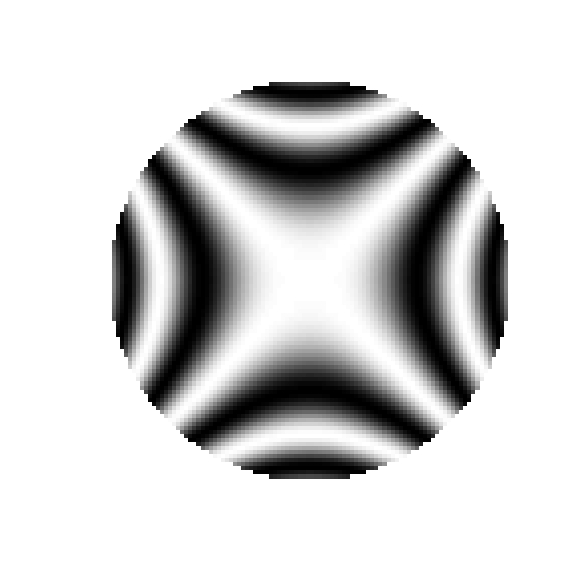
\includegraphics[width=0.06\textwidth]{Figures/conoscopy/table/00_90}&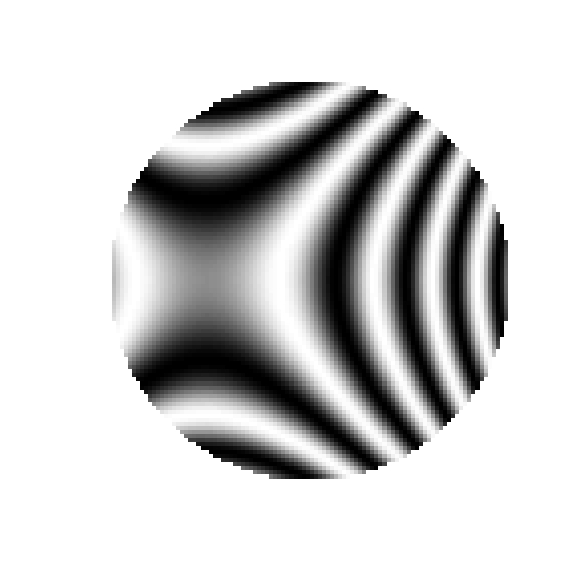
\includegraphics[width=0.06\textwidth]{Figures/conoscopy/table/00_85}&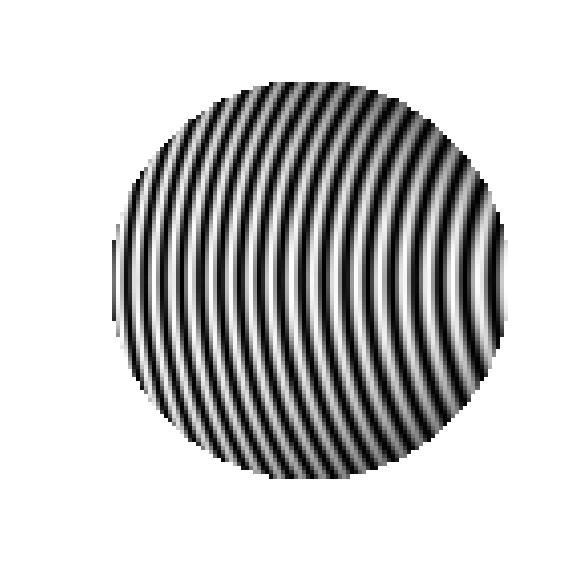
\includegraphics[width=0.06\textwidth]{Figures/conoscopy/table/00_45}&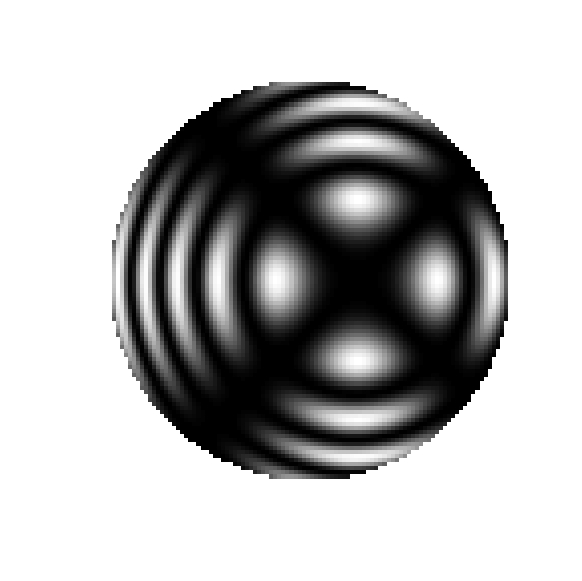
\includegraphics[width=0.06\textwidth]{Figures/conoscopy/table/00_05}&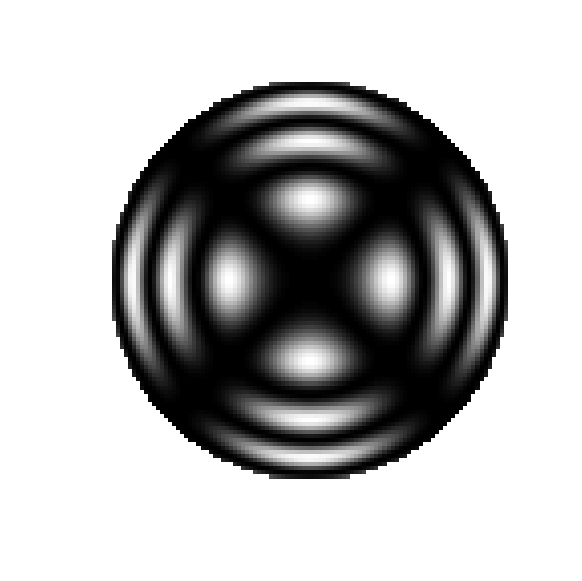
\includegraphics[width=0.06\textwidth]{Figures/conoscopy/table/00_00}\\
\end{tabular}
\caption[Characteristic conoscopic figures]{\label{fig:figures}A table showing characteristic conoscopic figures for varying values of $\theta$ and $\phi$ from the optical simulation package. Note that the polarisers are set at $\phi+45^{\circ}$, otherwise some of the figures in the $\theta>0$ column would appear nearly or entirely black. This accounts for the rotation of the $\theta=0$ figure, which would be independent of $\phi$ if the polariser angle did not change.}
\end{table}
\end{center}

Here as expected, for planar alignment $\left(\theta=90^{\circ}\right)$, the conjugate set of hyperbolae centred on a common locus is computed. This set of hyperbolae is rotated as a function of the azimuthal alignment, $\phi$ relative to the figure's $x$ axis. For pure vertical alignment $\left(\theta=0^{\circ}\right)$, the concentric circular fringes and maltese cross are computed. As stated earlier, for small uniform tilt angles away from either planar or vertical alignment $\left(\theta=85^{\circ},5^{\circ}\right)$, the locus of the simulated conoscopic figure appears slightly displaced from the centre of the field of view along a line parallel to the plane containing the director azimuthal alignment angle $\phi$.

\subsection{Experimental}
Figure \ref{fig:conoscope_schem} is a schematic diagram of the experimental set up that constitutes the conoscope used for analysis in this thesis. Here it is seen that firstly, light from a Helium-Neon laser (633 nm) is incident onto a rotating diffuser, acting as a scattering near point source over the small area illuminated by the beam spot. As the diffuser is rotated, the array of point sources varies, and when averaged over a single rotation of the diffuser, creates a uniform cone of light, removing any speckle pattern from the laser and final conoscopic figures. The beam is then collimated before passing through the first polariser and into the first microscope objective of the main assembly.

%\begin{figure}
%\begin{center}
%\subfigure[Experimental conoscope setup]{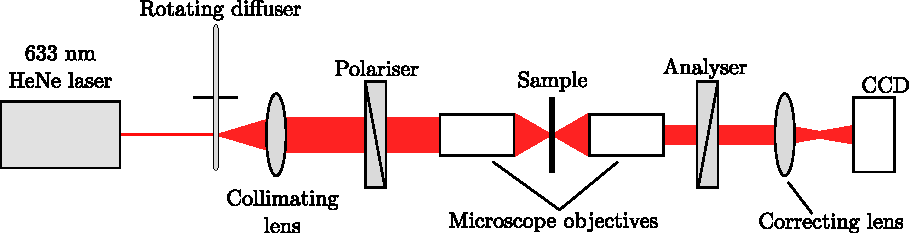
\includegraphics[width=\textwidth]{Figures/conoscopy/conoscope_setup}}\vspace{1cm}
%\subfigure[Magnification of cell in beam]{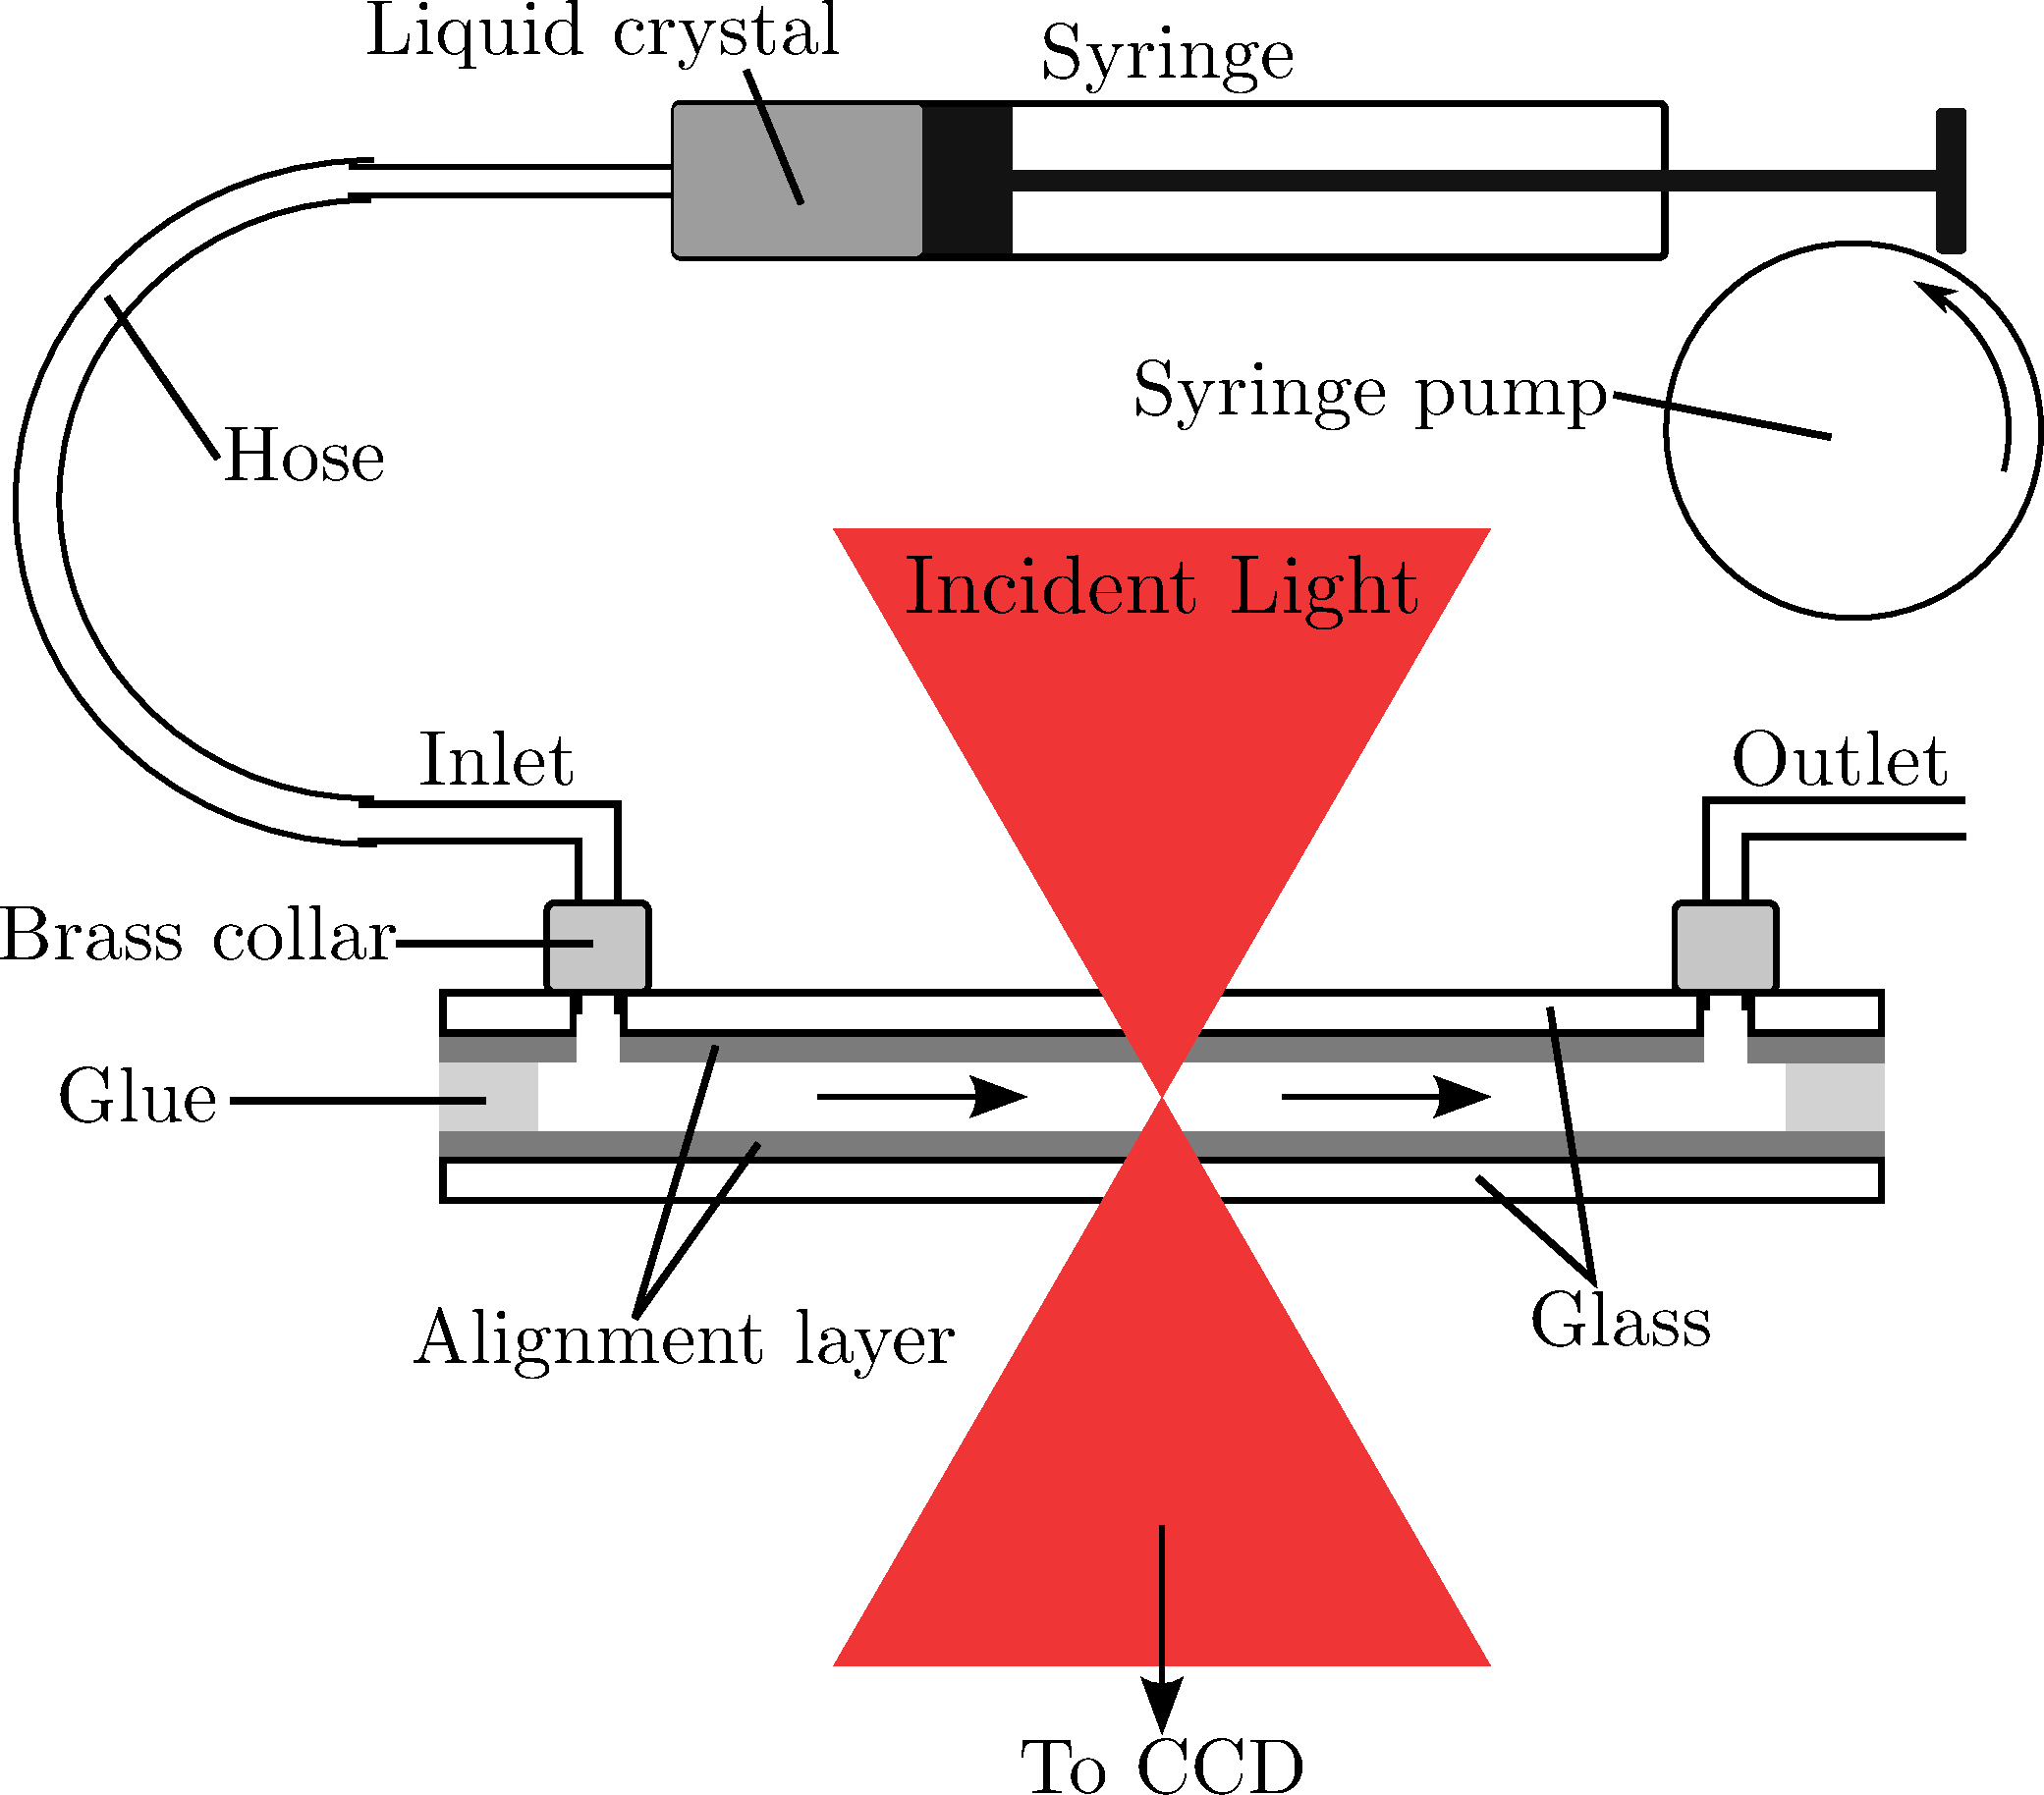
\includegraphics[width=0.6\textwidth]{Figures/Theory/cell_cono}}
%\end{center}
%\caption{\label{fig:conoscope_schem}(a)A schematic diagram of the conoscope used in this research. Based on a designs from the literature \cite{Parry-Jones2002,Fujikawa1993} and built by Cornford in reference \cite{Cornford2008}. Here, a collimated beam passes through the polariser, main assembly and sample, before passing through the analyser and focussed on to the CCD to capture a figure. (b) A magnification of a characteristic liquid crystal flow cell in the main assembly.}
%\end{figure}

\begin{figure}
\begin{center}
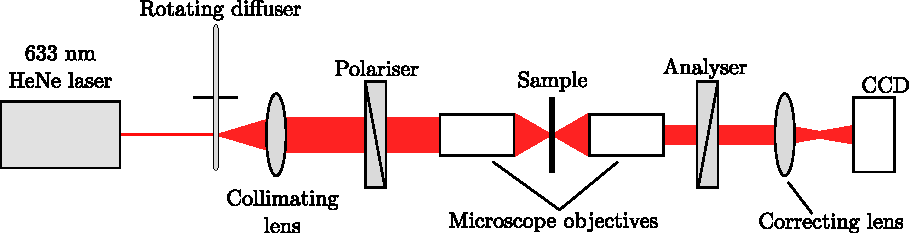
\includegraphics[width=0.48\textwidth]{Figures/conoscopy/conoscope_setup}
\end{center}
\caption[Schematic diagram of the conoscope setup]{\label{fig:conoscope_schem}A schematic diagram of the conoscope used in this research. Based on a designs from the literature \cite{Parry-Jones2002,Fujikawa1993} and built by Cornford in reference \cite{Cornford2008}. Here, a collimated beam passes through the polariser, main assembly and sample, before passing through the analyser and focussed on to the CCD to capture a figure.}
\end{figure}

The main assembly consists of the sample and two Mitotouyo Plan-Apo 50$\times$ long working distance microscope objectives. The first objective takes a parallel beam of light about 3 mm in diameter, expands it, and focusses it on to the sample. The resulting convergent beam has a numerical aperture of 0.55, and a working distance of 13 mm. Having passed through the sample, the second objective collimates the beam before it passes through the second polariser, also known as the analyser.

Finally, the beam passes through a correcting lens to correct for the change in focus of the convergent beam that is generated by passing through the two thick glass plates of the sample. When the outer part of the beam exiting the second objective is parallel, the inner part is convergent (clearly visible as the beam is brighter in the centre than at the edges). On going through the correcting lens, the beam is uniform in a single plane, and that is the position where the CCD is placed \cite{Cornford2008}, creating a conoscopic figure which is captured from computer software for the camera used.

The following sub-sections will look at sample data images captured from the conoscope shown schematically in Figure \ref{fig:conoscope_schem}. It will show (primarily for planar aligned samples) how the conoscopic figures respond to variations in certain parameters of the experimental setup, such as rotating the samples in the main assembly and rotating the polariser and analyser whilst viewing the conoscopic figure. These figures are compared to the computed figures from the optical simulation in order to confirm that the model is behaving accurately in predicting the correct conoscopic figure. Whilst the main focus of the work in this chapter, and in this thesis as a whole, is concerned with planar and near-planar aligned samples, some vertically aligned samples are included here in order to show the characteristic conoscopic figures that can be obtained.

\subsection{Planar alignment - rotating the cell}
All planar conoscopic images included in the following sections are taken from the same liquid crystal cell which is filled with 5CB sandwiched between two glass plates spaced with un-stretched Parafilm (thickness of approximately 100 $\mu m$). The surface alignment layer is a rubbed polyimide. For all simulation, refractive indices for 5CB at a wavelength of 633 nm and 25 $^{\circ}$C are used as $n_o=1.531$ and $n_e=1.706$ taken from reference \cite{Li2005}.

Firstly, Figure \ref{fig:rotate_cell_data} shows how the planar conoscopic figure responds when the cell is physically rotated when in the conoscope. Here the polariser and analyser remain crossed at $0^\circ$ and $90^\circ$ to the image's $x$ axis whilst the cell is rotated in increments of approximately $5^\circ$. The rubbing direction is initially at $45^\circ$ to the figure's $x$ axis (Figure \ref{fig:rotate_cell_data} (a)). As the cell is rotated, the conjugate hyperbolae that make the conoscopic figure, clearly rotate until the rubbing direction becomes parallel to the polariser direction. In this position, the incident light sees only one refractive index of the liquid crystal, resulting in no average polarisation conversion of the incident light. As such, all rays arriving at the analyser are stopped and the field of view becomes completely dark (Figure \ref{fig:rotate_cell_data} (i)). The same effect is also seen when the rubbing direction is exactly perpendicular to the polariser. If the cell were to be rotated through $360^\circ$, this field of view will go dark four times in total, that is, whenever the director is parallel to either the polariser or analyser.

\begin{figure}
\begin{center}
\subfigure[]{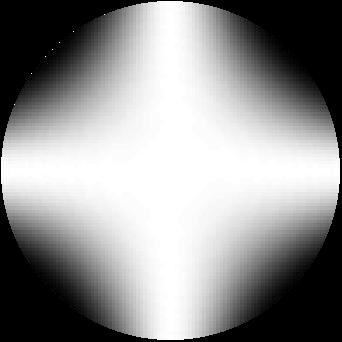
\includegraphics[width=0.1\textwidth]{Figures/conoscopy/Rotate_cell/00.jpg}}
\subfigure[]{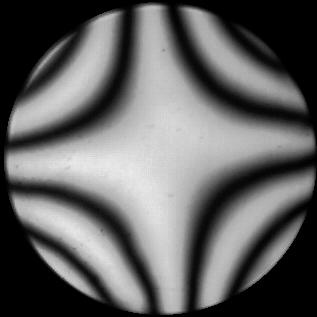
\includegraphics[width=0.1\textwidth]{Figures/conoscopy/Rotate_cell/01.jpg}}
\subfigure[]{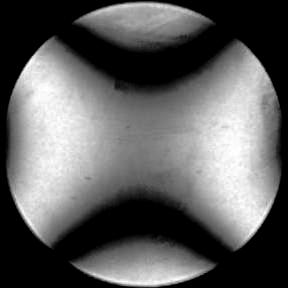
\includegraphics[width=0.1\textwidth]{Figures/conoscopy/Rotate_cell/02.jpg}}
\subfigure[]{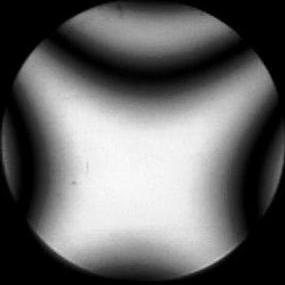
\includegraphics[width=0.1\textwidth]{Figures/conoscopy/Rotate_cell/03.jpg}}
\subfigure[]{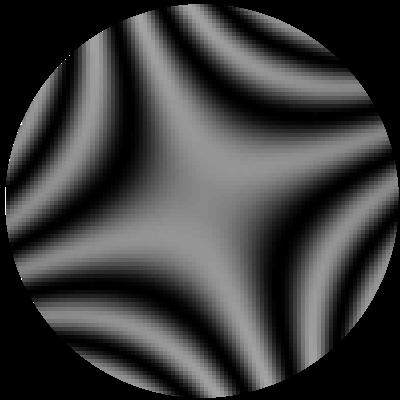
\includegraphics[width=0.1\textwidth]{Figures/conoscopy/Rotate_cell/04.jpg}}
\subfigure[]{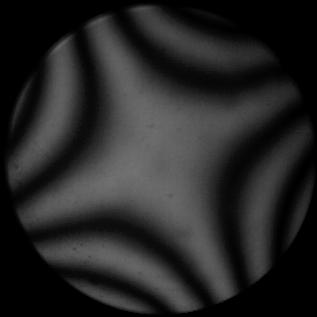
\includegraphics[width=0.1\textwidth]{Figures/conoscopy/Rotate_cell/05.jpg}}
\subfigure[]{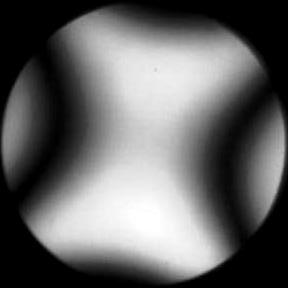
\includegraphics[width=0.1\textwidth]{Figures/conoscopy/Rotate_cell/06.jpg}}
\subfigure[]{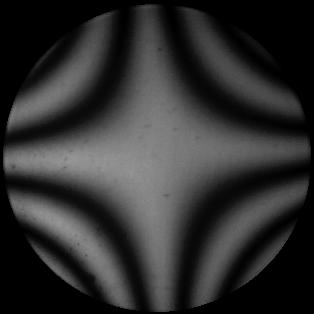
\includegraphics[width=0.1\textwidth]{Figures/conoscopy/Rotate_cell/07.jpg}}
\subfigure[]{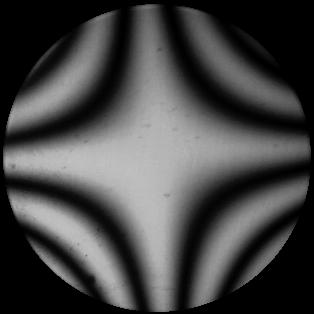
\includegraphics[width=0.1\textwidth]{Figures/conoscopy/Rotate_cell/08.jpg}}
\subfigure[]{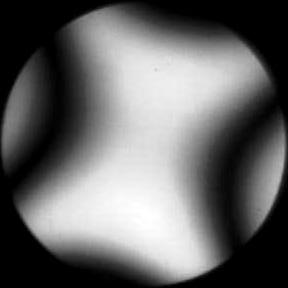
\includegraphics[width=0.1\textwidth]{Figures/conoscopy/Rotate_cell/09.jpg}}
\subfigure[]{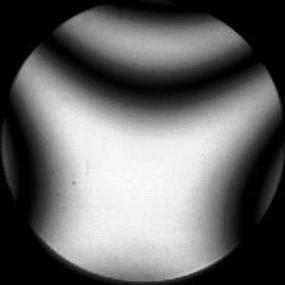
\includegraphics[width=0.1\textwidth]{Figures/conoscopy/Rotate_cell/10.jpg}}
\subfigure[]{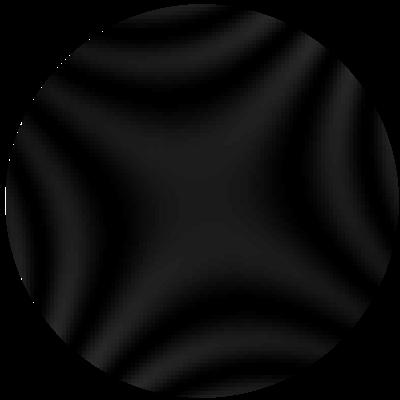
\includegraphics[width=0.1\textwidth]{Figures/conoscopy/Rotate_cell/11.jpg}}
\subfigure[]{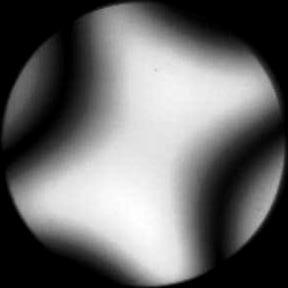
\includegraphics[width=0.1\textwidth]{Figures/conoscopy/Rotate_cell/12.jpg}}
\subfigure[]{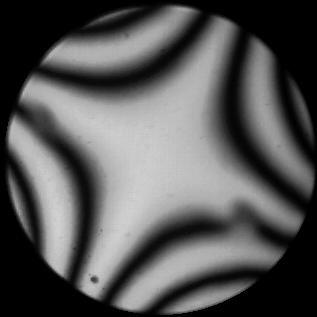
\includegraphics[width=0.1\textwidth]{Figures/conoscopy/Rotate_cell/13.jpg}}
\subfigure[]{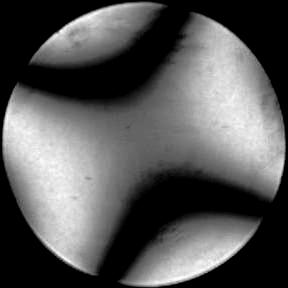
\includegraphics[width=0.1\textwidth]{Figures/conoscopy/Rotate_cell/14.jpg}}
\subfigure[]{\includegraphics[width=0.1\textwidth]{Figures/conoscopy/Rotate_cell/15.jpg}}
\subfigure[]{\includegraphics[width=0.1\textwidth]{Figures/conoscopy/Rotate_cell/16.jpg}}
\subfigure[]{\includegraphics[width=0.1\textwidth]{Figures/conoscopy/Rotate_cell/17.jpg}}
%\subfigure[]{\includegraphics[width=0.15\textwidth]{Figures/conoscopy/Rotate_cell/18.jpg}}
\end{center}
\caption[Conoscopic images of a planar cell - rotating]{\label{fig:rotate_cell_data}Data conoscopic figures for a planar aligned cell. The polariser and analyser remain crossed at $0^\circ$ and $90^\circ$ to the figure's $x$ axis whilst the cell is rotated in increments of approximately $5^\circ$ through images (a) to (r). When the cell is rotated so that the rubbing direction becomes parallel to either the polariser or analyser (image (i)), the field of view is shown to be  completely dark. This is due to the incident light experiencing only one of the refractive indices of the liquid crystal, resulting in no polarisation conversion and all light being blocked by the analyser.}
\end{figure}

Figure \ref{fig:rotate_cell_model} now shows the simulated conoscopic figures for the same experimental setup from which the conoscopic figures in Figure \ref{fig:rotate_cell_data} were obtained. This has been achieved by simulating the director profile to be aligned at varying azimuthal angles, whilst maintaining the polariser and analyser at $0^\circ$ and $90^\circ$ degrees respectively. It is clear that the uniaxial optics simulation provides very good agreement with the data obtained from the actual conoscope. As the azimuthal alignment of the director is changed, the field of view goes from showing the conjugate set of hyperbolae to going completely dark when the director and polariser or analyser are parallel with one another (Figure \ref{fig:rotate_cell_model} (i)).
 
\begin{figure}
\begin{center}
\subfigure[]{\includegraphics[width=0.1\textwidth]{Figures/conoscopy/Rotate_cell/modelled/cropped/01.jpg}}
\subfigure[]{\includegraphics[width=0.1\textwidth]{Figures/conoscopy/Rotate_cell/modelled/cropped/02.jpg}}
\subfigure[]{\includegraphics[width=0.1\textwidth]{Figures/conoscopy/Rotate_cell/modelled/cropped/03.jpg}}
\subfigure[]{\includegraphics[width=0.1\textwidth]{Figures/conoscopy/Rotate_cell/modelled/cropped/04.jpg}}
\subfigure[]{\includegraphics[width=0.1\textwidth]{Figures/conoscopy/Rotate_cell/modelled/cropped/05.jpg}}
\subfigure[]{\includegraphics[width=0.1\textwidth]{Figures/conoscopy/Rotate_cell/modelled/cropped/06.jpg}}
\subfigure[]{\includegraphics[width=0.1\textwidth]{Figures/conoscopy/Rotate_cell/modelled/cropped/07.jpg}}
\subfigure[]{\includegraphics[width=0.1\textwidth]{Figures/conoscopy/Rotate_cell/modelled/cropped/08.jpg}}
\subfigure[]{\includegraphics[width=0.1\textwidth]{Figures/conoscopy/Rotate_cell/modelled/cropped/09.jpg}}
\subfigure[]{\includegraphics[width=0.1\textwidth]{Figures/conoscopy/Rotate_cell/modelled/cropped/10.jpg}}
\subfigure[]{\includegraphics[width=0.1\textwidth]{Figures/conoscopy/Rotate_cell/modelled/cropped/11.jpg}}
\subfigure[]{\includegraphics[width=0.1\textwidth]{Figures/conoscopy/Rotate_cell/modelled/cropped/12.jpg}}
\subfigure[]{\includegraphics[width=0.1\textwidth]{Figures/conoscopy/Rotate_cell/modelled/cropped/13.jpg}}
\subfigure[]{\includegraphics[width=0.1\textwidth]{Figures/conoscopy/Rotate_cell/modelled/cropped/14.jpg}}
\subfigure[]{\includegraphics[width=0.1\textwidth]{Figures/conoscopy/Rotate_cell/modelled/cropped/15.jpg}}
\subfigure[]{\includegraphics[width=0.1\textwidth]{Figures/conoscopy/Rotate_cell/modelled/cropped/16.jpg}}
\subfigure[]{\includegraphics[width=0.1\textwidth]{Figures/conoscopy/Rotate_cell/modelled/cropped/17.jpg}}
\subfigure[]{\includegraphics[width=0.1\textwidth]{Figures/conoscopy/Rotate_cell/modelled/cropped/18.jpg}}
%\subfigure[]{\includegraphics[width=0.15\textwidth]{Figures/conoscopy/Rotate_cell/18.jpg}}
\end{center}
\caption[Simulated conoscopic images of a planar cell - rotating]{\label{fig:rotate_cell_model}Simulated conoscopic figures as the director azimuthal alignment is rotated in increments of $5^\circ$ from (a) to (r). These figures can be directly compared to the data conoscopic figures shown in Figure \ref{fig:rotate_cell_data} where a good agreement is seen.}
\end{figure}

\subsection{Planar alignment - rotating the polarisers}
A second experiment was also carried out, in which the cell was maintained in the same orientation (director at $45^\circ$ to the image's $x$ axis) but now, the polariser and analyser were rotated in $10^\circ$ increments whilst always remaining at $90^\circ$ to one another (crossed). The conoscopic figures obtained can be seen in Figure \ref{fig:stationary_cell_data}, images (a) to (j). As expected, the conjugate hyperbolae which make up the conoscopic figure remain undistorted, whilst the field of view gets darker before becoming completely black when either the polariser or analyser are aligned parallel to the rubbing direction (f). As the polariser and analyser are rotated past being parallel to the rubbing direction, the field of view becomes brighter again, returning to the initial conoscopic figure.

\begin{figure}
\begin{center}
\subfigure[]{\includegraphics[width=0.1\textwidth]{Figures/conoscopy/Stationary_cell/00.jpg}}
\subfigure[]{\includegraphics[width=0.1\textwidth]{Figures/conoscopy/Stationary_cell/01.jpg}}
\subfigure[]{\includegraphics[width=0.1\textwidth]{Figures/conoscopy/Stationary_cell/02.jpg}}
\subfigure[]{\includegraphics[width=0.1\textwidth]{Figures/conoscopy/Stationary_cell/03.jpg}}
\subfigure[]{\includegraphics[width=0.1\textwidth]{Figures/conoscopy/Stationary_cell/04.jpg}}
\subfigure[]{\includegraphics[width=0.1\textwidth]{Figures/conoscopy/Stationary_cell/05.jpg}}
\subfigure[]{\includegraphics[width=0.1\textwidth]{Figures/conoscopy/Stationary_cell/06.jpg}}
\subfigure[]{\includegraphics[width=0.1\textwidth]{Figures/conoscopy/Stationary_cell/07.jpg}}
\subfigure[]{\includegraphics[width=0.1\textwidth]{Figures/conoscopy/Stationary_cell/08.jpg}}
\subfigure[]{\includegraphics[width=0.1\textwidth]{Figures/conoscopy/Stationary_cell/09.jpg}}
\end{center}
\caption[Conoscopic images of a planar cell - rotating polarisers]{\label{fig:stationary_cell_data}Planar cell with the rubbing direction at at $45^\circ$ to the $x$ axis. The polariser and analyser remain crossed to one another whilst they are rotated in approximately $10^\circ$ increments from (a) to (j)}
\end{figure}

Figure \ref{fig:stationary_cell_model} again shows the simulated conoscopic figures for the same experimental set up, in which the alignment angle in the cell remains constant, and the polariser and analyser are rotated in $10^\circ$ increments whilst always remaining crossed to one another. Here again, it is clear that the uniaxial optics simulation provides very good agreement with the data obtained from the conoscope. As the polariser and analyser are rotated, the field of view goes from showing the conjugate set of hyperbolae to appearing completely dark when the director and polariser or analyser are parallel with each other (Figure \ref{fig:stationary_cell_model} (f)).

\begin{figure}
\begin{center}
\subfigure[]{\includegraphics[width=0.1\textwidth]{Figures/conoscopy/Stationary_cell/modelled/cropped/00.jpg}}
\subfigure[]{\includegraphics[width=0.1\textwidth]{Figures/conoscopy/Stationary_cell/modelled/cropped/01.jpg}}
\subfigure[]{\includegraphics[width=0.1\textwidth]{Figures/conoscopy/Stationary_cell/modelled/cropped/02.jpg}}
\subfigure[]{\includegraphics[width=0.1\textwidth]{Figures/conoscopy/Stationary_cell/modelled/cropped/03.jpg}}
\subfigure[]{\includegraphics[width=0.1\textwidth]{Figures/conoscopy/Stationary_cell/modelled/cropped/04.jpg}}
\subfigure[]{\includegraphics[width=0.1\textwidth]{Figures/conoscopy/Stationary_cell/modelled/cropped/05.jpg}}
\subfigure[]{\includegraphics[width=0.1\textwidth]{Figures/conoscopy/Stationary_cell/modelled/cropped/06.jpg}}
\subfigure[]{\includegraphics[width=0.1\textwidth]{Figures/conoscopy/Stationary_cell/modelled/cropped/07.jpg}}
\subfigure[]{\includegraphics[width=0.1\textwidth]{Figures/conoscopy/Stationary_cell/modelled/cropped/08.jpg}}
\subfigure[]{\includegraphics[width=0.1\textwidth]{Figures/conoscopy/Stationary_cell/modelled/cropped/09.jpg}}
\end{center}
\caption[Simulated conoscopic images of a planar cell - rotating polarisers]{\label{fig:stationary_cell_model}Simulated conoscopic figures whereby the polariser and analyser remain crossed to one another and are rotated in increments of $10^\circ$ from (a) to (j). These figures can be directly compared to the data conoscopic figures shown in Figure \ref{fig:stationary_cell_data} whereby a good agreement is seen.}
\end{figure}

\subsection{Planar alignment - thickness variation}
Figure \ref{fig:planar_thickness} demonstrates how the planar alignment conoscopic figure varies as a function of the cell thickness. The conoscopic figures in Figure \ref{fig:planar_thickness} were achieved by tracking across the cell in the $x-y$ plane with each image (a) to (g) taken at a different point. Here it is shown that the conjugate set of hyperbolae can move into and out of the centre of the conoscopic figure. As the cell thickness increases, there will be more fringes visible within the field of view. Conversely, as the cell thickness decreases, there will be fewer fringes in the field of view. This effect of cell thickness on fringe number is also true in the case of a vertically aligned sample (shown later in Figure \ref{fig:homeotropic_cell}), where extra sets of concentric circular fringes can be seen as the cell thickness increases. In Figure \ref{fig:planar_thickness}, the director is aligned at 45$^\circ$ to the figure's $x$ axis, and most importantly, there is very little change in this angle of orientation as the cell is moved around. This demonstrates that the rubbed polymer alignment layer has produced spatially coherent director alignment over a relatively large area (millimetres) of the cell. 

\begin{figure}
\begin{center}
\subfigure[]{\includegraphics[width=0.1\textwidth]{Figures/conoscopy/Planar_thickness/0}}
\subfigure[]{\includegraphics[width=0.1\textwidth]{Figures/conoscopy/Planar_thickness/1.jpg}}
\subfigure[]{\includegraphics[width=0.1\textwidth]{Figures/conoscopy/Planar_thickness/2.jpg}}
\subfigure[]{\includegraphics[width=0.1\textwidth]{Figures/conoscopy/Planar_thickness/3.jpg}}
\subfigure[]{\includegraphics[width=0.1\textwidth]{Figures/conoscopy/Planar_thickness/4.jpg}}
\subfigure[]{\includegraphics[width=0.1\textwidth]{Figures/conoscopy/Planar_thickness/5.jpg}}
\subfigure[]{\includegraphics[width=0.1\textwidth]{Figures/conoscopy/Planar_thickness/6.jpg}}
\end{center}
\caption[Conoscopic images of thickness variations in a planar cell]{\label{fig:planar_thickness}Conoscopic interference figure for a planar cell rubbed at 45$^\circ$ to the figure's $x$ axis. Polariser and analyser are crossed and at 0$^\circ$ and 90$^\circ$ to the figure's $x$ axis. Figures (a) through (g) show how the figure changes when moving the cell approximately 5 mm in the x-direction due to a depth gradient across the cell.}
\begin{center}
%\rule{3in}{0.5pt}
\end{center}
\end{figure}

\subsection{Vertical alignment}
Figure \ref{fig:homeotropic_cell} shows captured conoscopic figures for a cell that has been aligned vertically through a surface treatment of lecithin dissolved in ether\footnote{In order to achieve a good alignment layer, a small amount of lecithin is dissolved in the ether until the solution becomes pale yellow in colour. The face is then coated by dragging a lens tissue soaked in the solution across the glass surface.}. Here it is shown that the conoscopic figure consists of (as described earlier) concentric circular fringes and a central extinction cross that is often referred to as the `classic' maltese cross. Figure \ref{fig:homeotropic_cell} (a) and (b) show captured conoscopic figures for the same vertically aligned cell whereby the polariser and analyser are crossed $0^\circ$ and $90^\circ$ to the $x$ axis, and at $45^\circ$ and $135^\circ$ to the $x$ axis respectively. This difference in polariser/analyser alignment is shown by the rotation of the extinction cross through $45^\circ$. Figures \ref{fig:homeotropic_cell} (c) and (d) show two conoscopic figure captures from a different cell, in which a thickness gradient exists. Much like in the case of the planar conoscopic figure example (Figure \ref{fig:planar_thickness}) the number of concentric circular fringes visible at the edge of the field of view increases as the cell becomes thicker. This is visible when looking at image (c) with just one set of fringes and image (d) which contains two sets of fringes\footnote{The slight displacement of the locus from the centre of the field of view in Figure \ref{fig:homeotropic_cell} (c) and (d) when compared with (a) and (b) suggests that the director may be slightly tilted away from vertical alignment}.


\begin{figure}
\begin{center}
\subfigure[]{\includegraphics[width=0.1\textwidth]{Figures/conoscopy/homeotropic/00.jpg}}
\subfigure[]{\includegraphics[width=0.1\textwidth]{Figures/conoscopy/homeotropic/01.jpg}}\\
\subfigure[]{\includegraphics[width=0.1\textwidth]{Figures/conoscopy/homeotropic/03.jpg}}
\subfigure[]{\includegraphics[width=0.1\textwidth]{Figures/conoscopy/homeotropic/04.jpg}}
\end{center}
\caption[Conoscopic figures from a vertically aligned cell]{\label{fig:homeotropic_cell}Data conoscopic figure captures of a a cell aligned vertically through a surface treatment of lecithin dissolved in ether. Figures (a) and (b) show figures where the crossed polarisers are at $0^{\circ}$ and $45^{\circ}$ to the $x$ axis respectively. Figures (c) and (d) depict a vertically aligned cell whereby (d) is captured in a slightly thicker part of the cell, with more fringes visible around the maltese cross.}
\end{figure}

\subsection{Polarisers crossed and parallel}
Finally, Figure \ref{fig:pol_crossed_parallel} shows a comparison between planar aligned and vertically aligned captured conoscopic figures viewed when the polariser and analyser are crossed to one another (a) and (c) and also when the analyser has been rotated to become parallel to the polariser (b) and (d). These figures were again captured as a test to see whether the conoscope was working as expected. For both cases, the conoscopic figures captured when the polariser and analyser are parallel to one another appear to be the inverse of the figures where the polariser and analyser are crossed to one another. This is as expected. When the analyser is rotated to be parallel to the polariser, any light that exits the cell polarised orthogonal to the analyser will be blocked, resulting in a dark area on the conoscopic figure. When the analyser is rotated through $90^{\circ}$ to be parallel to the polariser, this same light will be passed by the analyser, resulting in a light area on the conoscopic figure. This is shown by Figure \ref{fig:pol_crossed_parallel} (b) now having a dark centre, and most strikingly the inverse vertically aligned conoscopic figure whereby a light cross is formed by four dark lobes.

\begin{figure}
\begin{center}
\subfigure[]{\includegraphics[width=0.1\textwidth]{Figures/conoscopy/polarisers/00.jpg}}
\subfigure[]{\includegraphics[width=0.1\textwidth]{Figures/conoscopy/polarisers/01.jpg}}\\
\subfigure[]{\includegraphics[width=0.1\textwidth]{Figures/conoscopy/polarisers/02.jpg}}
\subfigure[]{\includegraphics[width=0.1\textwidth]{Figures/conoscopy/polarisers/03.jpg}}
\end{center}
\caption[Conoscopic images when polarisers are crossed and parallel]{\label{fig:pol_crossed_parallel}A comparison between data conoscopic figures for a planar aligned cell and a vertically aligned cell viewed when the polariser and analyser are crossed to one another and also when they are parallel to one another. Images (a) and (b) show a planar aligned cell viewed conoscopically between crossed and parallel polarisers respectively. Images (c) and (d) show a vertically aligned cell viewed conoscopically between crossed and parallel polarisers respectively. In both cases, the conoscopic figures are essentially the inverse of the original.}
\end{figure}

\subsection{Tracking conoscopic figure alignment}
In order to accurately determine the alignment angle of the conjugate hyperbolae present in the planar conoscopic figure, a computer minimisation routine was created to automatically iterate down to the correct angle. Typical output figures from this program can be seen in Figure \ref{fig:figure_rotation1}. Before the automated routine can be run, the conoscopic figures must be lightly processed in order for them to work with the computer program. This processing involves cropping the images to be square, and smoothing the figures to remove any artefacts that may give misleading results (simple gaussian smoothing in ImageJ is suitable for this). Examples of an original simulated planar conoscopic figure and the smoothed version can be seen in Figure \ref{fig:figure_rotation1} (a) and (b). 

In order to accurately determine the angle at which the hyperbolae are aligned, the program plots an initial line running through the centre of the field of view at a pre-defined angle (normally measured from the $x$ axis of the figure). Two further test lines are then plotted parallel and at a fixed distance to the initial line. The automated routine then plots the values of the pixel intensities along these two test lines and plots them as a function of position along the test line. Pairs of images can be seen in Figure \ref{fig:figure_rotation1} (c) to (j) in which the test lines plotted on the conoscopic figure (left column) correspond to the pixel intensities as a function of position on the line (plotted in the right column). The program then alters the angle at which the initial line is plotted (each time re-plotting two new parallel test lines) and measuring the difference between the pixel intensities for this given initial line. The automated routine varies the initial line angle to iterate down to a line which best minimises the difference in sum of the pixel intensities between the two test lines. At this point, the angle of the plotted line defines the angle at which the conjugate hyperbolae of the conoscopic figure are aligned.

For example, Figure \ref{fig:figure_rotation1} (c) shows the initial line and the two test lines plotted either side for the first iteration. It is clear by eye that the initial guess does not minimise the difference in pixel intensities of the two lines, although this is confirmed in (d) whereby the pixel intensities along the test lines in image (c) are plotted. It is clearly visible that the data points and line do not overlap each other. The second iteration (images (e) and (f)) make the situation even worse, with a bigger difference between the plotted pixel intensities. Accordingly, the third iteration moves the test line in the opposite direction ((g) and (h)) and a smaller difference between the test line pixel intensities is found. After the fourth iteration, the difference between the test line pixel intensities is minimised ((i) and (j)) and the angle at which the test lines are plotted over the conoscopic figure is returned by the program. In practice, this process may take more than four iterations, but is a valuable tool in systematically and automatically ascertaining the alignment angle of the conjugate hyperbolae of the planar conoscopic figure.

As will be seen in later chapters, the fits between the plotted pixel intensities are far worse when the automated routine is carried out on actual conoscopic figures as opposed to here where the simulated noise-free figures provide easy minimisation and near perfect evaluation of the alignment angle.

\begin{figure}
\begin{center}
\subfigure[Original]{\includegraphics[width=0.15\textwidth]{Figures/Mirror/bob}}\hspace{0.4cm}
\subfigure[Smoothed]{\includegraphics[width=0.15\textwidth]{Figures/Mirror/bobsmooth}}\\
\scalebox{0.9}[1]{\subfigure[]{\includegraphics[width=0.2\textwidth]{Figures/Mirror/1}}}
\scalebox{0.9}[1]{\subfigure[]{\includegraphics[width=0.2\textwidth]{Figures/Mirror/2}}}\\
\scalebox{0.9}[1]{\subfigure[]{\includegraphics[width=0.2\textwidth]{Figures/Mirror/3}}}
\scalebox{0.9}[1]{\subfigure[]{\includegraphics[width=0.2\textwidth]{Figures/Mirror/4}}}\\
\scalebox{0.9}[1]{\subfigure[]{\includegraphics[width=0.2\textwidth]{Figures/Mirror/5}}}
\scalebox{0.9}[1]{\subfigure[]{\includegraphics[width=0.2\textwidth]{Figures/Mirror/6}}}\\
\scalebox{0.9}[1]{\subfigure[]{\includegraphics[width=0.2\textwidth]{Figures/Mirror/9}}}
\scalebox{0.9}[1]{\subfigure[]{\includegraphics[width=0.2\textwidth]{Figures/Mirror/10}}}
\end{center}
\caption[Automated conoscopic figure tracking routine]{\label{fig:figure_rotation1}(a) Original simulated conoscopic figure. (b) Original figure after smoothing in ImageJ. Images (c) to (j) show pairs of images whereby the pixel intensities plotted along the two lines either side of the central test line are plotted. After three iterations, the difference between the left and right test lines has been minimised resulting in determination of the azimuthal alignment angle of the conoscopic figure.}
\end{figure}

This chapter will now go on to discuss the cell fabrication methods developed during this study in order to conduct the pressure driven flow experiments that will be detailed in the following chapters.

\subsection{Cell fabrication}
\label{sec:cell_fabrication}
In order to conduct dynamic pressure driven flow experiments, robust cells that allow flow of a liquid crystal from a syringe drive must be fabricated. During the course of this investigation, a set technique has been developed, refined and improved upon, to become what is now a standard process for the production of pressure driven flow cells within the group at Exeter.

Cells are generally constructed from a standard glass microscope slide that has been cut in half to produce two approximately 3 cm by 2 cm plates. One of the plates is drilled with holes by our workshop technicians to allow for the inlet/outlet pipes to be attached. The plates are then cleaned (see below), before having a surface alignment layer deposited, and rubbed if necessary.

\subsection{Microscope slide preparation}
\begin{enumerate}
\item 
All cleaning of microscope slides and cover slips is carried out in clean tents, where fans perpetually circulate the air in the immediate environment. All processes are also carried out wearing latex gloves to minimise contamination with skin grease or other foreign bodies from the immediate environment.
\item 
Slides are removed from their sealed container and firstly cleaned rigorously with a cotton bud soaked in acetone. Initially they are rubbed with firm pressure in one direction and then rubbed again at 90$^{\circ}$ to the initial cleaning direction. This technique is considered to be a mechanical cleaning process to get rid of any debris or small particles that may be on the surface of the slide. The acetone also aids in removing any grease or smudges that are present on the slides\footnote{One must take care not to use the same end of the cotton bud twice as this can result in contamination of the solvent reservoir}.
\item 
Step 2 is then repeated with cotton buds soaked in isopropanol (IPA). This step removes any residue left by the acetone on the surface of the slide. The slides are then blasted with an inert dusting gas to remove any fibres that may have been left by the cotton buds.
\item 
Finally, and most importantly, the slides are drag cleaned with lens tissue soaked in IPA. The lens tissue is placed over the slide and pulled slowly (at approximately the same rate that the IPA evaporates) across the slide with tweezers. This process removes any smears or debris left by the previous stages. This step can be repeated several times until the slide is free of any defects when examined by eye.
\end{enumerate}

\subsection{Cell construction}
\label{sec:cell_construction}
At this stage, aligning layers can be deposited onto the glass slides. Conventionally this is done by spin coating a layer of polyimide in order to align the director, whereby the particular composition of the polymer promotes a particular alignment. Once the glass slides have been prepared with an alignment layer, they are ready to be brought together to form a flow cell. Figure \ref{fig:cell_fabrication} shows a schematic diagram of this process. 

\begin{figure}
\begin{center}
\includegraphics[width=0.49\textwidth]{Figures/45/cell_fabrication}
\end{center}
\caption[Cell fabrication]{\label{fig:cell_fabrication}(a) The glass slides are placed on a clean and flat surface ready for cell construction. (b) Stretched strips of \textit{Parafilm} are placed either side of the inlet/outlet holes to define a flow channel. (c) The plates are sandwiched together and the excess \textit{Parafilm} is removed. The cell is then placed on a hot plate to bond the  \textit{Parafilm} to the glass. (d) UV curing glue is introduced to seal the channel ends and cured under a UV lamp. (e) Inlet and outlet pipes are attached to the flow cell with an epoxy resin adhesive.}
\end{figure}

\begin{enumerate}
\item 
Firstly, the slides are placed on a flat clean surface and arranged so that the top plate can be placed on top of the bottom plate to create the initial alignment conditions required.
\item
Two thin strips of \textit{Parafilm} are cut and stretched by hand to form the walls of the flow channel. Prior to stretching, the \textit{Parafilm} is approximately 120 $\mu$m thick, once stretched, this is reduced to approximately 45 $\mu$m. These strips are placed on either side of the inlet and outlet holes, defining a flow channel that is approximately 3 mm in width. The two slides are then sandwiched together under a moderate pressure. The surplus pieces of \textit{Parafilm} are removed with a scalpel.
\item
The cell is placed on a hot plate at approximately 60 $^{\circ}$C, or until the \textit{Parafilm} becomes tacky and bonds the two glass plates together. During this time, a cotton bud can be used to apply pressure to the \textit{Parafilm} walls, flattening and aiding the bonding process.
\item
A UV curing glue (Norland optical adhesive) is applied by a cocktail stick to the open ends of the flow channel. This then capillary fills into the cell. Great care must be taken to apply only a very small amount of glue to the cell, as it can fill too far up the flow channel and block either the inlet or outlet hole. The cell is then placed under a UV lamp for approximately 15 minutes, or until the glue has cured.
\item
Finally, steel inlet (and outlet if necessary) tubes are glued to the cell with an epoxy resin. To aid the bonding process, the bottom surface of the brass collar surrounding the inlet/outlet tube can be roughened with a file or scalpel. The advent of brass collars to secure the pipe to the cell at the inlet and outlet holes has been a key development in fabricating robust and well sealed flow cells, as shown in Figure \ref{fig:collar}. In some cases, the area of the glass cell around the inlet hole can be masked off and roughened with an air sand blaster. This process can aid the strength of the bonding between the collar and the glass.
\end{enumerate}

A diagram showing a typical flow cell in relation to the syringe drive and conoscope for the experiments described in the following chapters is given in Figure \ref{fig:conoscope_schem1}. The flow cell is connected to a syringe pump and is placed at the convergent point of the cone of light in the conoscope.

\begin{figure}
\begin{center}
\subfigure[]{\includegraphics[width=0.2\textwidth]{Figures/45/collar_photo}}\hspace{0.5in}
\subfigure[]{\includegraphics[width=0.2\textwidth]{Figures/45/collar}}
\end{center}
\caption[Flow cell connections]{\label{fig:collar}(a) Shows a photograph of epoxy resin being applied to a collar with a cocktail stick. (b) A schematic diagram of the collar on the pipe as it is inserted into a slide. The collar and glue form a robust contact around the joint ensuring there is no leakage.}
\end{figure}

\begin{figure}
\begin{center}
\includegraphics{Figures/Theory/cell_cono}
\end{center}
\caption[Schematic depiction of flow cell in the conoscope]{\label{fig:conoscope_schem1} A schematic representation of a flow cell in relation to the syringe drive and convergent part of the conoscopic beam.}
\end{figure}

